\documentclass[a4paper,10pt]{article}

\usepackage[T1]{fontenc}
\usepackage[utf8]{inputenc}
\usepackage[french]{babel}
\usepackage{lmodern}
\usepackage[margin=1.6cm,top=1.4cm,bottom=1.3cm]{geometry}
\usepackage{booktabs}
\usepackage{graphicx}
\usepackage{amsmath}
\usepackage{amssymb}
\usepackage{xcolor}
\usepackage[colorlinks=true,urlcolor=blue!55!black,linkcolor=black]{hyperref}
\usepackage{titlesec}
\usepackage{enumitem}

\graphicspath{{figures/}}

\titlespacing*{\section}{0pt}{1.5ex plus .2ex}{0.5ex}
\titlespacing*{\subsection}{0pt}{1.1ex plus .2ex}{0.4ex}
\titleformat{\section}{\normalfont\large\bfseries}{\thesection.}{0.5em}{}
\titleformat{\subsection}{\normalfont\bfseries}{\thesubsection.}{0.5em}{}
\setlist[itemize]{leftmargin=1.1em,itemsep=0.1ex,topsep=0.2ex,parsep=0pt}
\setlength{\parskip}{0.3ex}
\setlength{\parindent}{0pt}
\pagestyle{empty}

\newcommand{\pc}[1]{#1\,\%}
\newcommand{\etat}[1]{{\footnotesize\textsf{[#1]}}}
\newcommand{\expfig}[1]{%
  \begin{minipage}[c]{0.375\textwidth}
    \includegraphics[width=\linewidth]{#1}
  \end{minipage}\hfill}
\newcommand{\exptxt}[1]{%
  \begin{minipage}[c]{0.605\textwidth}#1\end{minipage}\\[0.6ex]}

\begin{document}

\begin{center}
  {\large\bfseries Psychophysique de la détection des perturbations internes dans les LLM~:
   introspection, anomalie ou géométrie~?}\\[0.4ex]
  {\small Note technique --- Llama-3.1-8B-Instruct \quad|\quad Sujet 15, F.~Popineau}
\end{center}

\section{Problématique}

Hahami et al.~\href{https://arxiv.org/abs/2512.12411}{\NoAutoSpacing(arXiv:2512.12411)} montrent qu'un modèle
open-weight de 8B sait dire \emph{où} son calcul a été perturbé et \emph{laquelle} de deux
perturbations était la plus forte. Fornasiere et al.~({\NoAutoSpacing arXiv:2604.17465}) montrent que cette capacité
n'est pas réservée aux modifications porteuses de sens~: le dropout et le bruit gaussien sont
détectés eux aussi. D'où l'ambiguïté d'interprétation~: \textbf{le modèle reconnaît-il la
\emph{nature} de ce qui a changé dans son état interne, ou seulement qu'une activation est
inhabituelle~?}

La réponse dépend d'un choix de mesure rarement explicité~: \textbf{comment quantifier la \og force\fg{}
d'une perturbation}. Les activations d'un LLM ne varient pas de la même façon dans toutes les
directions~; une même amplitude numérique $\alpha$ peut être banale selon une direction et très
anormale selon une autre. Comparer concept, direction aléatoire et bruit \emph{à $\alpha$ apparié}
revient donc à comparer des perturbations qui ne sont pas de même intensité \emph{pour le modèle},
et toute différence de détectabilité observée peut n'être qu'un artefact de paramétrisation.

Nos runs préliminaires en donnent une illustration directe. Sur la comparaison d'intensité, une
grille de dropout plafonnée à $p \leq 0{,}6$ donnait \pc{65} au mieux --- lecture~: \og le dropout ne
supporte pas la tâche\fg{}. Rejouée sur $p \in [0{,}6\,;\,0{,}9]$, c'est-à-dire de l'autre côté du pied
de la courbe dose-réponse, la même tâche donne \pc{90}, \emph{au-dessus} des vecteurs de concept
(\pc{83,8}). La grille mesurait la grille, pas le modèle. Comme le dropout rééchelonné a une
variance de bruit par entrée en $p/(1-p)$, la grille initiale ne couvrait qu'un $\sigma$ relatif de
$0{,}33$ à $1{,}22$ alors que le seuil se situe au-delà.

\medskip
\textbf{Question de recherche.} Lorsqu'on compare des perturbations conceptuelles, aléatoires et
bruitées, observe-t-on les mêmes différences de détectabilité selon que leur intensité est mesurée
(i)~par l'amplitude brute de l'injection $\alpha$, (ii)~par son importance relative aux variations
naturelles des activations, $z = \alpha / s(\ell, v)$, ou (iii)~par son effet sur la sortie du
modèle~? L'approche est celle de la psychophysique computationnelle~: courbes psychométriques
complètes, seuil à \pc{75}, choix forcé à deux alternatives (2AFC) utilisé comme
\emph{instrument de mesure} et non comme résultat, sans assimiler l'auto-rapport à une forme de
conscience.

\section{Plan}

\begin{itemize}
  \item[] \textbf{Partie 1 --- Reproduction de Hahami et al.} \etat{fait, \S\,3}\\
        Prise en main du dépôt et des hooks~; vecteurs de concept~; les trois tâches
        (détection binaire, comparaison d'intensité, localisation) rejouées et confrontées aux
        chiffres publiés. Sert de calibration de l'instrument, pas de contribution.
  \item[] \textbf{Partie 2 --- Normalisation de l'intensité} \etat{à faire}\\
        Estimation de $s(\ell, v)$ au même hook que l'injection, sur corpus témoin et positions de
        tokens éligibles~; écart-type en analyse principale, MAD robuste en sensibilité~;
        diagnostic des distributions d'activations par couche et par direction.
  \item[] \textbf{Partie 3 --- Courbes psychométriques} \etat{à faire}\\
        Sweep principal à $z$ apparié, analyse parallèle à $\alpha$ apparié~; concept /
        direction aléatoire / bruit gaussien / dropout~; seuil \pc{75}, $d'$ si justifié,
        bootstrap hiérarchique par concept et par paire.
  \item[] \textbf{Partie 4 --- Robustesse et contrôles} \etat{à faire}\\
        Effet de couche~; ordre contrebalancé et distance inter-phrases contrôlée en 2AFC~;
        diagnostic de contamination phrase~1 $\rightarrow$ phrase~2~; concepts hold-out~;
        comparaison explicite des conclusions entre paramétrisations.
  \item[] \textbf{Partie 5 --- Extensions} \etat{si budget}\\
        Appariement aval par divergence KL/JS sur un sous-ensemble, comme analyse de sensibilité~;
        second modèle open-weight $\leq$ 8B, seulement si le résultat principal est stabilisé.
\end{itemize}

\section{Partie 1 --- Reproduction de Hahami et al.}

\subsection{Vecteurs de concept}

Dix concepts, deux constructions~: pour les cinq concepts simples (\emph{Dust}, \emph{Satellites},
\emph{Trumpets}, \emph{Origami}, \emph{Illusions}),
$v_\ell = a_\ell(\text{mot}) - \frac{1}{50}\sum_b a_\ell(b)$ sur 50 mots de référence~; pour les cinq
complexes (\emph{appreciation}, \emph{betrayal}, \emph{fibonacci\_numbers}, \emph{recursion},
\emph{shutdown}), $v_\ell = \overline{a_\ell(\text{pos})} - \overline{a_\ell(\text{neg})}$ sur
$20+20$ phrases. $a_\ell$ = moyenne des états cachés de la couche $\ell$ sur les tokens du prompt.
Injection~: $v$ normalisé, $h \leftarrow h + \alpha v$ en sortie de couche $\ell$, sur les seuls
tokens de la phrase ciblée, hooks retirés avant la génération. Les trois tâches ne diffèrent que par
le prompt et la métrique. C'est aussi ce hook qui portera $s(\ell, v)$ en Partie~2.

\subsection{Détection binaire --- \textit{\og as-tu détecté une pensée injectée en \textsc{sentence}~1\,?\fg{}}}

\expfig{detection_concept.png}
\exptxt{
\centering
\small
\begin{tabular}{@{}lcc@{}}
\toprule
& \textbf{Hahami et al.} & \textbf{Nous} \\
\midrule
L0 (tous $\alpha$) & \pc{88,7} & \pc{97,6} \\
L4--L8             & \pc{55,4} & \pc{57,3} \\
L12--L30           & \pc{50,6} & \pc{55,0} \\
\bottomrule
\end{tabular}

\vspace{0.7ex}
\raggedright
\footnotesize
8 couches $\times$ 5 $\alpha$ $\times$ 100 essais. Métrique~:
$\Delta L_{\text{adj}} = \Delta L_{\text{brut}} - \Delta L_{\text{base}}$.
\textbf{La moins évidente des trois}, car l'accuracy brute est de \pc{0,02} (2 essais sur 8\,880)~:
tout repose sur la constante de base. Elle doit être mesurée \emph{avec le protocole du sweep} ---
\texttt{run\_position\_detection()} met le prompt en cache puis réinjecte le dernier token, déjà
présent. Ce décalage de $+0{,}139 \pm 0{,}121$ logit vaut $\sim$\,30 points d'accuracy en couches
profondes. Mesurée ainsi, notre base vaut $-3{,}139 \pm 0{,}263$ ($n=200$) et la Table~1 se
reproduit. Deux contrôles~: la base indépendante du dépôt de référence ($-3{,}317 \pm 0{,}329$)
concorde, tandis que les $-3{,}96$ publiés saturent toutes les cellules à \pc{100} --- ce que fait
effectivement le \texttt{table1.csv} des auteurs ($\geq\!\pc{98}$ dans les 40 cellules).
La conclusion de leur Section~4 tient~: effet de couche~0, décalage global de la distribution de
sortie, pas d'introspection.
}

\subsection{Comparaison d'intensité --- quelle phrase a été perturbée le plus fort~?}

\expfig{intensite_concept.png}
\exptxt{
\centering
\small
\begin{tabular}{@{}lcc@{}}
\toprule
& \textbf{Hahami et al.} & \textbf{Nous} \\
\midrule
L3, paire $(3,7)$   & \pc{83} & \pc{83,8} \\
moyenne L15--L30    & \pc{47} & \pc{47,3} \\
\bottomrule
\end{tabular}

\vspace{0.7ex}
\raggedright
\footnotesize
15 couches $\times$ 4 paires $\times$ 300 essais~; hasard \pc{50}. Deux phrases injectées à
$\alpha_1 \neq \alpha_2$, les deux ordres testés pour neutraliser le biais de position, ajusté sur
la ligne de base sans injection de chaque couche.
\textbf{Reproduction exacte}~: même couche de pic (L3), même paire de pic $(3,7)$, même valeur au
pic et même queue plate à partir de L15. Un décalage global vers un token de réponse ne peut pas
aider ici --- il faut désigner \emph{laquelle} des deux positions a été touchée le plus fort.
C'est le protocole 2AFC qui servira d'instrument en Parties~3 et~4.
}

\subsection{Localisation --- laquelle des dix phrases a été perturbée~?}

\expfig{localisation_concept.png}
\exptxt{
\centering
\small
\begin{tabular}{@{}lcc@{}}
\toprule
& \textbf{Hahami et al.} & \textbf{Nous} \\
\midrule
L2, $\alpha=5$ & \pc{88} & \pc{96,6} \\
L3, $\alpha=5$ & \pc{76} & \pc{73,7} \\
L4, $\alpha=8$ & \pc{65} & \pc{63,1} \\
\bottomrule
\end{tabular}

\vspace{0.7ex}
\raggedright
\footnotesize
11 couches $\times$ 7 $\alpha$ $\times$ 500 essais~; hasard \pc{10}. Contenu des phrases tenu
constant et perturbation cyclée sur les dix positions, donc indices de contenu et biais de position
contrôlés~; aucun ajustement de base n'est nécessaire.
Deux des trois cellules citées tombent à 2--3 points près, la troisième ressort plus haut. La forme
de leur Figure~2 --- pic précoce puis effondrement au-delà de L8 --- est retrouvée intégralement,
l'effondrement étant même plus net (L11+ au niveau du hasard ou en dessous).
}

\subsection{Bilan de la Partie 1}

Les trois tâches se reproduisent numériquement, y compris la plus fragile une fois le protocole de
ligne de base aligné. L'instrument est donc calibré et le pipeline fiable~: conformément au cadrage
du sujet, la réplication s'arrête ici et le travail bascule sur la contribution originale
(Parties~2--4). Le code repart des utilitaires et scripts d'expérience du dépôt des auteurs,
\href{https://github.com/elyhahami18/llama-introspection-new}{\texttt{github.com/elyhahami18/llama-introspection-new}}.


\section{Partie 2 --- Calibration de l'échelle naturelle}

\subsection{Expérience 0 --- objectif et périmètre}

Cette expérience estime la variabilité naturelle des activations dans les
directions qui seront utilisées lors des interventions, sans injection et sans
réponse comportementale. Le corpus comprend 100 phrases de
\texttt{LOCALIZATION\_SENTENCES}, soit 616 positions admissibles, observées à la
sortie des 32 blocs Transformer.

Trois familles sont calibrées : les dix directions conceptuelles, dix directions
aléatoires fixes par couche et une direction de bruit renouvelé par couche et
position admissible. Cela représente respectivement 320, 320 et 19\,712 couples
couche--direction, soit 20\,352 estimations au total. Les directions aléatoires
fixes sont persistées pour être réutilisées ; les directions de bruit sont
régénérables à partir de graines distinctes. Aucune dose $\alpha$ ou $z$ et
aucune perturbation dropout ne sont calculées à cette étape.
\subsection{Calcul détaillé de l'échelle $s(\ell,v)$}

Soit $\mathcal{X}=\{x_1,\ldots,x_J\}$ le corpus témoin, avec $J=100$ phrases.
Pour chaque phrase $x_j$, on note $\mathcal{T}_j$ l'ensemble des positions de
tokens admissibles. Le nombre total d'observations est
\[
N=\sum_{j=1}^{J}|\mathcal{T}_j|=616.
\]
Chaque couple $(j,t)$, avec $t\in\mathcal{T}_j$, constitue une observation.
Les tokens ont le même poids dans l'estimation ponctuelle : aucune moyenne par
phrase n'est effectuée avant le calcul de l'échelle.

\paragraph{Extraction des activations.}

Chaque phrase est passée dans le modèle sans intervention. Pour chaque bloc
Transformer $\ell\in\{0,\ldots,31\}$ et chaque position admissible $t$, on
extrait
\[
h_{\ell,j,t}\in\mathbb{R}^{d},
\]
où $d=4096$ est la dimension résiduelle de Llama-3.1-8B-Instruct.
L'activation est prélevée à la sortie du bloc $\ell$, c'est-à-dire exactement
au futur site d'injection.

Les activations $h_{\ell,j,t}$ ne sont pas normalisées. Elles sont produites
par le modèle en \texttt{bfloat16}, puis converties en \texttt{float32} pour
la projection. Les statistiques finales sont calculées en \texttt{float64}.

\paragraph{Normalisation des directions.}

Pour chaque couche $\ell$ et chaque direction brute
$u_{\ell,v}\in\mathbb{R}^{d}$, on construit une direction unitaire
\[
v_{\ell}
=
\frac{u_{\ell,v}}
     {\lVert u_{\ell,v}\rVert_2},
\qquad
\lVert v_{\ell}\rVert_2=1.
\]
Cette normalisation est appliquée aux trois familles :

\begin{itemize}
  \item les vecteurs de concept ;
  \item les directions aléatoires fixes ;
  \item les directions de bruit renouvelé.
\end{itemize}

Pour les deux familles isotropes, le vecteur brut est tiré selon
\[
u_{\ell,v}\sim\mathcal{N}(0,I_d),
\]
puis normalisé. Les directions aléatoires fixes sont conservées dans une banque
persistante, tandis que les directions de bruit renouvelé utilisent une graine
distincte pour chaque couche et position cible. La norme originale
$\lVert u_{\ell,v}\rVert_2$ est enregistrée pour la traçabilité, mais elle
n'intervient pas dans le calcul de $s(\ell,v)$.

\paragraph{Projections naturelles.}

Pour chaque activation admissible, on calcule sa projection scalaire sur la
direction unitaire :
\[
p_{j,t}(\ell,v)
=
\left\langle h_{\ell,j,t},v_{\ell}\right\rangle
=
\sum_{k=1}^{d}h_{\ell,j,t,k}\,v_{\ell,k}.
\]
Pour un couple $(\ell,v)$ donné, on obtient donc l'échantillon
\[
\mathcal{P}_{\ell,v}
=
\left\{
p_{j,t}(\ell,v)
\;\middle|\;
j\in\{1,\ldots,J\},\;
t\in\mathcal{T}_j
\right\},
\]
qui contient $N=616$ projections.

La moyenne des projections est
\[
\overline{p}_{\ell,v}
=
\frac{1}{N}
\sum_{j=1}^{J}
\sum_{t\in\mathcal{T}_j}
p_{j,t}(\ell,v).
\]

\paragraph{Échelle principale : écart-type.}

L'échelle principale est l'écart-type échantillonnal des projections :
\[
\boxed{
s_{\mathrm{SD}}(\ell,v)
=
\sqrt{
\frac{1}{N-1}
\sum_{j=1}^{J}
\sum_{t\in\mathcal{T}_j}
\left(
p_{j,t}(\ell,v)-\overline{p}_{\ell,v}
\right)^2
}
}
\]
Le dénominateur est $N-1$, conformément à l'estimation échantillonnale
(\texttt{ddof=1}). Cette quantité mesure la variabilité globale des activations
naturelles dans la direction $v$.

Comme $v$ est unitaire mais que $h_{\ell,j,t}$ ne l'est pas,
$s_{\mathrm{SD}}(\ell,v)$ conserve l'amplitude naturelle des activations dans
cette orientation. Normaliser également les activations transformerait la
projection en une mesure principalement angulaire et supprimerait une partie
de l'information d'amplitude recherchée.

\paragraph{Échelle robuste : MAD corrigée.}

On calcule d'abord la médiane des projections :
\[
m_{\ell,v}
=
\operatorname{médiane}_{j,t}
\left[p_{j,t}(\ell,v)\right].
\]
La déviation absolue médiane est ensuite
\[
\operatorname{MAD}(\ell,v)
=
\operatorname{médiane}_{j,t}
\left[
\left|
p_{j,t}(\ell,v)-m_{\ell,v}
\right|
\right].
\]
La version corrigée utilisée dans l'expérience est
\[
\boxed{
s_{\mathrm{MAD}}(\ell,v)
=
1{,}4826\,
\operatorname{médiane}_{j,t}
\left[
\left|
p_{j,t}(\ell,v)-m_{\ell,v}
\right|
\right]
}
\]
Le facteur $1{,}4826$ place la MAD sur la même échelle que la SD lorsque les
projections suivent une distribution gaussienne. Contrairement à la SD, la MAD
décrit principalement la largeur de la région centrale de la distribution et
est peu influencée par des observations très éloignées.

Le rapport
\[
R(\ell,v)
=
\frac{s_{\mathrm{SD}}(\ell,v)}
     {s_{\mathrm{MAD}}(\ell,v)}
\]
sert de diagnostic :

\begin{itemize}
  \item $R(\ell,v)\simeq 1$ indique que les deux mesures d'échelle sont
        comparables ;
  \item $R(\ell,v)\gg 1$ indique que la dispersion globale mesurée par la SD
        est beaucoup plus grande que la dispersion centrale mesurée par la MAD.
\end{itemize}

Un rapport élevé peut notamment apparaître lorsque les projections mélangent
plusieurs groupes de tokens ou de phrases, présentent plusieurs modes, ou
contiennent des observations éloignées. Il ne permet pas, à lui seul, de choisir
la meilleure normalisation.

\paragraph{Bootstrap par phrase.}

L'incertitude de $s(\ell,v)$ est estimée par bootstrap en conservant la phrase
comme unité de rééchantillonnage. Pour chaque réplication $b$, on tire avec
remise $J=100$ phrases :
\[
x^{(b)}_1,\ldots,x^{(b)}_J
\sim
\operatorname{ÉchantillonnageAvecRemise}(\mathcal{X}).
\]
Lorsqu'une phrase est tirée, toutes ses positions admissibles sont conservées.
Si elle est tirée plusieurs fois, l'ensemble de ses tokens est répété avec la
même multiplicité. On obtient ainsi un multiensemble d'observations
$\mathcal{I}^{(b)}$ de taille
\[
N_b
=
\sum_{j=1}^{J}
M_j^{(b)}|\mathcal{T}_j|,
\]
où $M_j^{(b)}$ désigne le nombre de fois où la phrase $x_j$ a été tirée.

Pour chaque réplication, on recalcule
\[
s_{\mathrm{SD}}^{(b)}(\ell,v)
=
\sqrt{
\frac{1}{N_b-1}
\sum_{(j,t)\in\mathcal{I}^{(b)}}
\left(
p_{j,t}(\ell,v)
-
\overline{p}_{\ell,v}^{(b)}
\right)^2
}
\]
et, de façon analogue,
\[
s_{\mathrm{MAD}}^{(b)}(\ell,v)
=
1{,}4826\,
\operatorname{médiane}_{(j,t)\in\mathcal{I}^{(b)}}
\left|
p_{j,t}(\ell,v)-m_{\ell,v}^{(b)}
\right|.
\]

Le calcul utilise :

\begin{itemize}
  \item $B_{\mathrm{SD}}=1000$ réplications pour la SD ;
  \item $B_{\mathrm{MAD}}=200$ réplications pour la MAD ;
  \item des intervalles empiriques à \pc{95}, donnés par les quantiles
        $2{,}5$ et $97{,}5$ des estimations bootstrap.
\end{itemize}

La stabilité relative est résumée par le coefficient de variation bootstrap :
\[
\operatorname{CV}_{\mathrm{SD}}(\ell,v)
=
\frac{
\operatorname{SD}_{b}
\left[
s_{\mathrm{SD}}^{(b)}(\ell,v)
\right]
}{
\operatorname{moyenne}_{b}
\left[
s_{\mathrm{SD}}^{(b)}(\ell,v)
\right]
},
\]
avec la même définition pour $\operatorname{CV}_{\mathrm{MAD}}$.

\paragraph{Valeurs conservées.}

Pour chaque couple $(\ell,v)$, la calibration enregistre donc
\[
\left(
\overline{p}_{\ell,v},
\;
m_{\ell,v},
\;
s_{\mathrm{SD}}(\ell,v),
\;
s_{\mathrm{MAD}}(\ell,v),
\;
q_{0{,}01},
\;
q_{0{,}05},
\;
q_{0{,}95},
\;
q_{0{,}99}
\right),
\]
ainsi que les intervalles bootstrap, les coefficients de variation, la famille
de la direction, sa provenance, sa graine et sa norme originale.

Une valeur peut servir à la normalisation SD ultérieure si
\[
s_{\mathrm{SD}}(\ell,v)>0.
\]
Les 20\,352 couples couche--direction du calcul actuel satisfont cette
condition.

Cette calibration permettra ultérieurement de convertir une intensité
standardisée $z$ en amplitude d'injection :
\[
\alpha_{\mathrm{SD}}(\ell,v,z)
=
z\,s_{\mathrm{SD}}(\ell,v),
\]
ou, dans l'analyse de sensibilité robuste,
\[
\alpha_{\mathrm{MAD}}(\ell,v,z)
=
z\,s_{\mathrm{MAD}}(\ell,v).
\]
Ces conversions ne sont pas encore appliquées dans l'expérience~0 : celle-ci
calcule uniquement les échelles naturelles nécessaires aux expériences
comportementales suivantes.


Remplace toute la sous-section envoyée par celle-ci. J’ai gardé la figure, le tableau et les chiffres, mais organisé l’interprétation avec des paragraphes thématiques.

```latex
\subsection{Dépendance à la couche et à la direction}

\begin{center}
  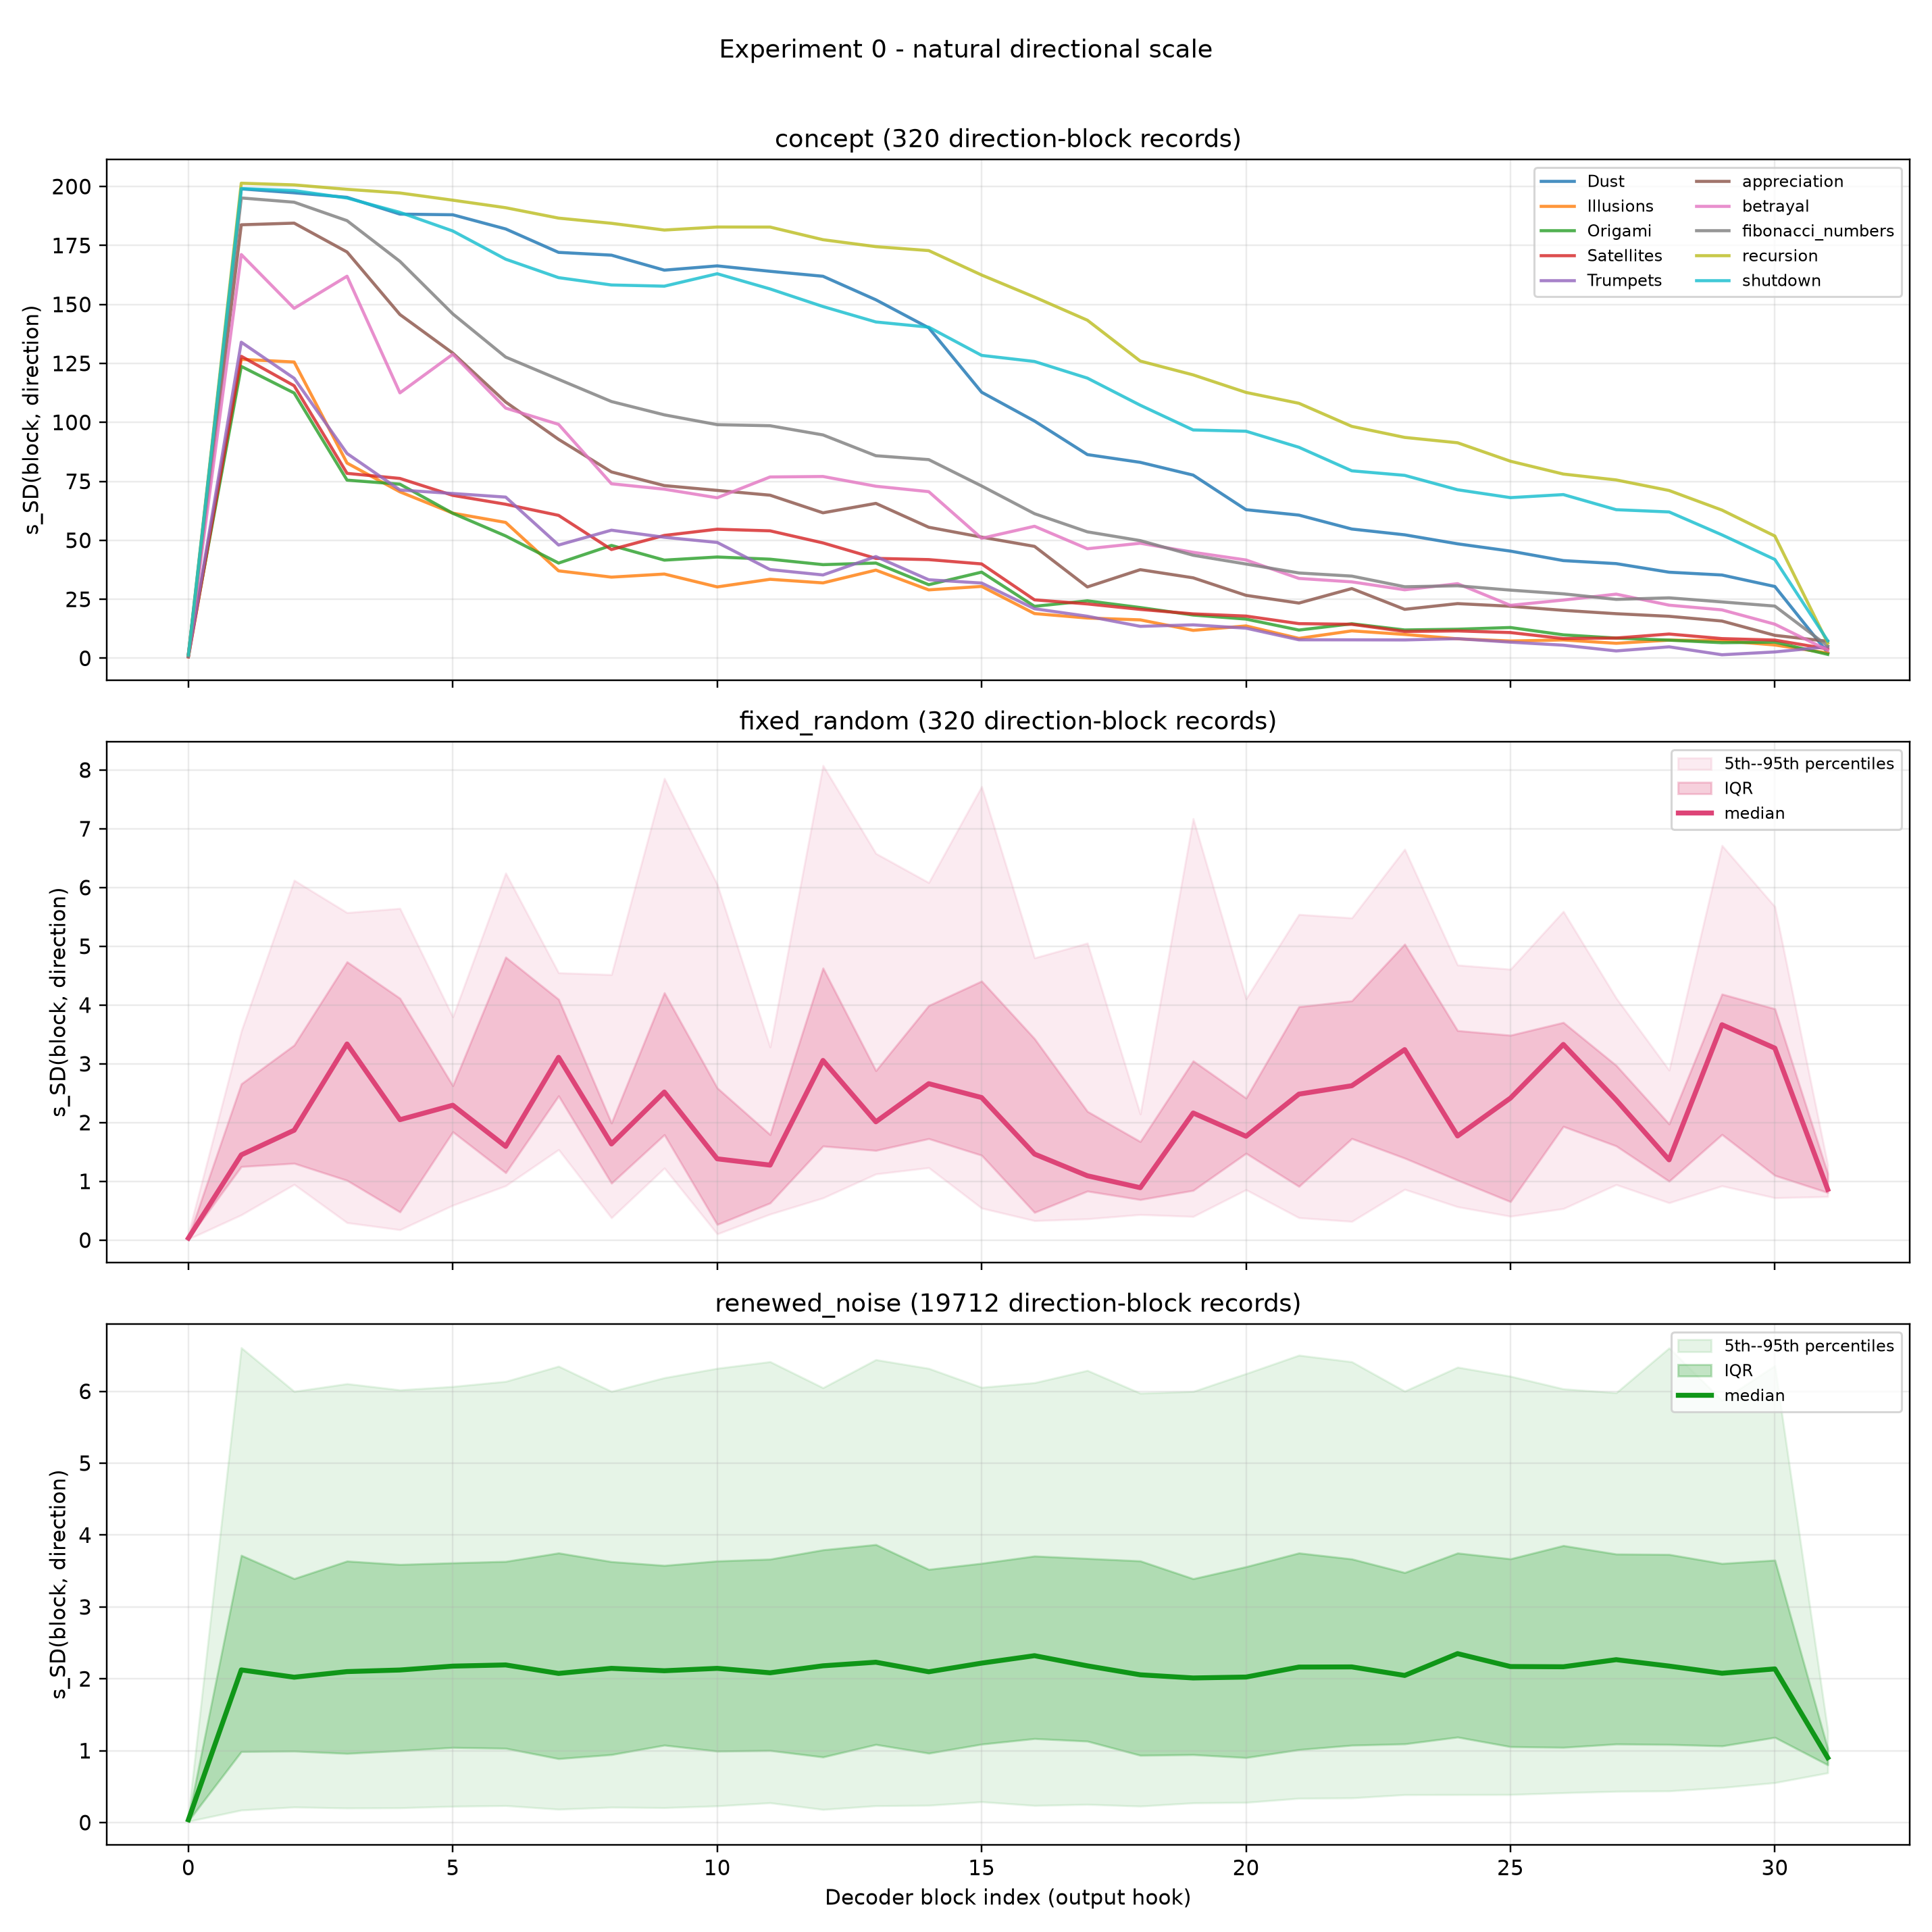
\includegraphics[width=0.48\textwidth]{experiment_0_scales_sd.png}
  \par\vspace{0.3ex}
  {\footnotesize
  Échelles $s_{\mathrm{SD}}(\ell,v)$ selon la couche. Les concepts sont
  représentés individuellement ; pour les directions aléatoires fixes et le
  bruit renouvelé, la ligne indique la médiane, la bande sombre l'IQR et la
  bande claire les quantiles 5--95\,\%.\par}
\end{center}

\begin{center}
  \small
  \begin{tabular}{@{}rccc@{}}
    \toprule
    $\ell$ & concepts & aléatoires fixes & bruit renouvelé \\
    \midrule
     0 & $1{,}19$  & $0{,}033$ & $0{,}039$ \\
     1 & $177{,}5$ & $1{,}45$  & $2{,}12$  \\
    16 & $51{,}7$  & $1{,}46$  & $2{,}32$  \\
    30 & $12{,}1$  & $3{,}27$  & $2{,}14$  \\
    31 & $4{,}40$  & $0{,}86$  & $0{,}90$  \\
    \bottomrule
  \end{tabular}

  \vspace{0.4ex}
  {\footnotesize
  Médiane de $s_{\mathrm{SD}}(\ell,v)$ entre les directions de chaque famille,
  pour cinq couches représentatives.\par}
\end{center}

\paragraph{Effet de la couche.}

L'échelle naturelle varie fortement le long du réseau. Les trois familles
présentent une hausse nette entre les blocs 0 et 1. Dans les couches suivantes,
la médiane des échelles conceptuelles diminue progressivement, tandis que les
directions aléatoires fixes et le bruit renouvelé restent généralement dans un
intervalle de l'ordre de $1$ à $3$, avant de diminuer au dernier bloc. Une même
amplitude brute $\alpha$ ne correspond donc pas à une intensité naturelle
constante d'une couche à l'autre.

Il faut toutefois préciser que les courbes ne suivent pas une direction unique
à travers tout le modèle. À chaque couche $\ell$ correspond une direction
$v_\ell$ construite ou tirée dans l'espace de cette couche. Les différences
entre couches reflètent ainsi simultanément l'évolution des activations du
modèle et celle des directions sur lesquelles elles sont projetées.

\paragraph{Pourquoi les concepts ont-ils une échelle plus élevée ?}

Toutes les directions étant normalisées à norme $1$, l'écart observé ne vient
pas d'une différence de longueur entre les vecteurs. Il vient de leur
\emph{orientation} dans l'espace des activations.

Pour une direction unitaire $v$, l'échelle vérifie
\[
s_{\mathrm{SD}}^2(\ell,v)
=
v^\top\widehat{\Sigma}_{\ell}v,
\]
où $\widehat{\Sigma}_{\ell}$ est la covariance des activations naturelles à la
couche $\ell$. Cette expression signifie simplement que $s(\ell,v)$ mesure la
quantité de variabilité des activations portée par l'orientation $v$.

Une direction aléatoire pointe vers une orientation quelconque dans un espace
de dimension $4096$. Elle mesure donc généralement une variabilité
directionnelle ordinaire ou moyenne. Une direction conceptuelle est au
contraire construite à partir de différences d'activations du modèle :
\[
u_{\ell,c}
=
\overline{h}_{\ell,c^{+}}
-
\overline{h}_{\ell,c^{-}},
\qquad
v_{\ell,c}
=
\frac{u_{\ell,c}}{\lVert u_{\ell,c}\rVert_2}.
\]
Elle est ainsi directement déterminée par la géométrie interne du modèle. Elle
peut s'aligner avec des axes le long desquels les activations naturelles varient
beaucoup plus que dans une direction choisie au hasard. Dans ce cas,
\[
s(\ell,v_{\mathrm{concept}})
\gg
s(\ell,v_{\mathrm{aléatoire}}).
\]

C'est ce que montrent les résultats. Au bloc~1, la médiane conceptuelle vaut
$177{,}5$, contre $1{,}45$ pour les directions aléatoires fixes et $2{,}12$
pour le bruit renouvelé. Elle est donc environ $122$ fois plus élevée que la
médiane aléatoire. Ce rapport reste proche de $35$ au bloc~16, puis diminue
jusqu'à environ $3{,}7$ au bloc~30. L'alignement particulier des concepts avec
les axes de forte variabilité est donc surtout marqué dans les couches
précoces et intermédiaires.

Cette interprétation reste géométrique : elle ne prouve pas que toute la
variabilité supplémentaire est exclusivement sémantique. Les vecteurs de
concept peuvent également être alignés avec des propriétés lexicales, certains
types de tokens, leur position ou d'autres régularités présentes dans leurs
données de construction. La calibration montre que ces directions sont
atypiques par rapport à des directions isotropes, mais elle ne détermine pas
encore la cause exacte de cette particularité.

\paragraph{Pourquoi les directions aléatoires et le bruit sont-ils proches ?}

Les directions aléatoires fixes et les directions de bruit renouvelé sont
construites de la même manière :
\[
g\sim\mathcal N(0,I_d),
\qquad
v=\frac{g}{\lVert g\rVert_2}.
\]
Après normalisation, elles suivent donc la même distribution isotrope sur
l'espace des activations. Il est alors attendu que leurs échelles naturelles
soient du même ordre. Par exemple, leurs médianes respectives valent $1{,}45$
et $2{,}12$ au bloc~1, puis $1{,}46$ et $2{,}32$ au bloc~16.

Ces deux familles se distinguent par leur utilisation, et non par leur nature
géométrique :

\begin{itemize}
  \item les dix directions aléatoires fixes de chaque couche constituent une
        banque de contrôles qui sera réutilisée dans plusieurs essais ;
  \item le bruit renouvelé utilise une direction indépendante pour chaque
        couche et chaque position cible.
\end{itemize}

Le nombre beaucoup plus élevé de directions de bruit améliore la description
statistique de cette famille, mais ne lui donne pas plus de poids dans le calcul
d'un $s(\ell,v)$ individuel. Chaque direction, quelle que soit sa famille, est
projetée sur les mêmes 616 activations du corpus témoin. Dans les figures, les
directions de bruit sont ensuite résumées par leur médiane et leurs quantiles,
afin que leur nombre ne domine pas artificiellement la comparaison.

\paragraph{Hétérogénéité au sein des concepts.}

Les dix concepts ne présentent pas la même échelle. Au bloc~16,
$s_{\mathrm{SD}}$ vaut environ $19$ à $25$ pour \emph{Illusions},
\emph{Origami}, \emph{Satellites} et \emph{Trumpets}, contre $101$ pour
\emph{Dust}, $126$ pour \emph{shutdown} et $153$ pour \emph{recursion}. Au
bloc~30, les valeurs s'étendent encore d'environ $2{,}7$ pour
\emph{Trumpets} à $51{,}8$ pour \emph{recursion}.

Il ne serait donc pas correct d'utiliser une unique échelle moyenne pour tous
les concepts. La conversion future devra être effectuée séparément pour chaque
couple couche--concept :
\[
\alpha(\ell,v,z)=z\,s(\ell,v).
\]
La comparaison entre concepts simples et complexes devra également rester
prudente, car leurs vecteurs n'ont pas été construits avec les mêmes données ni
avec le même type de contraste. Une différence d'échelle peut refléter la
géométrie du concept, sa méthode de construction, ou une combinaison des deux.

\paragraph{Conséquence pour l'appariement des perturbations.}

À amplitude brute égale, une perturbation conceptuelle représente généralement
une fraction beaucoup plus faible de la variabilité naturelle correspondante :
\[
z(\ell,v)=\frac{\alpha}{s(\ell,v)}.
\]
Au bloc~1, par exemple, la forte différence de $s$ implique qu'un même
$\alpha$ produit un $z$ environ $122$ fois plus faible pour la direction
conceptuelle médiane que pour la direction aléatoire médiane.

Inversement, imposer le même $z$ nécessitera une amplitude absolue plus élevée
dans les directions dont l'échelle naturelle est grande. Les résultats
confirment ainsi que les comparaisons comportementales devront être présentées
à la fois à $\alpha$ apparié et à $z$ apparié : la première conserve l'amplitude
numérique de l'intervention, tandis que la seconde contrôle son importance
relativement à la variabilité naturelle de chaque couche et direction.
```

\subsection{Divergence entre SD et MAD}

\begin{center}
  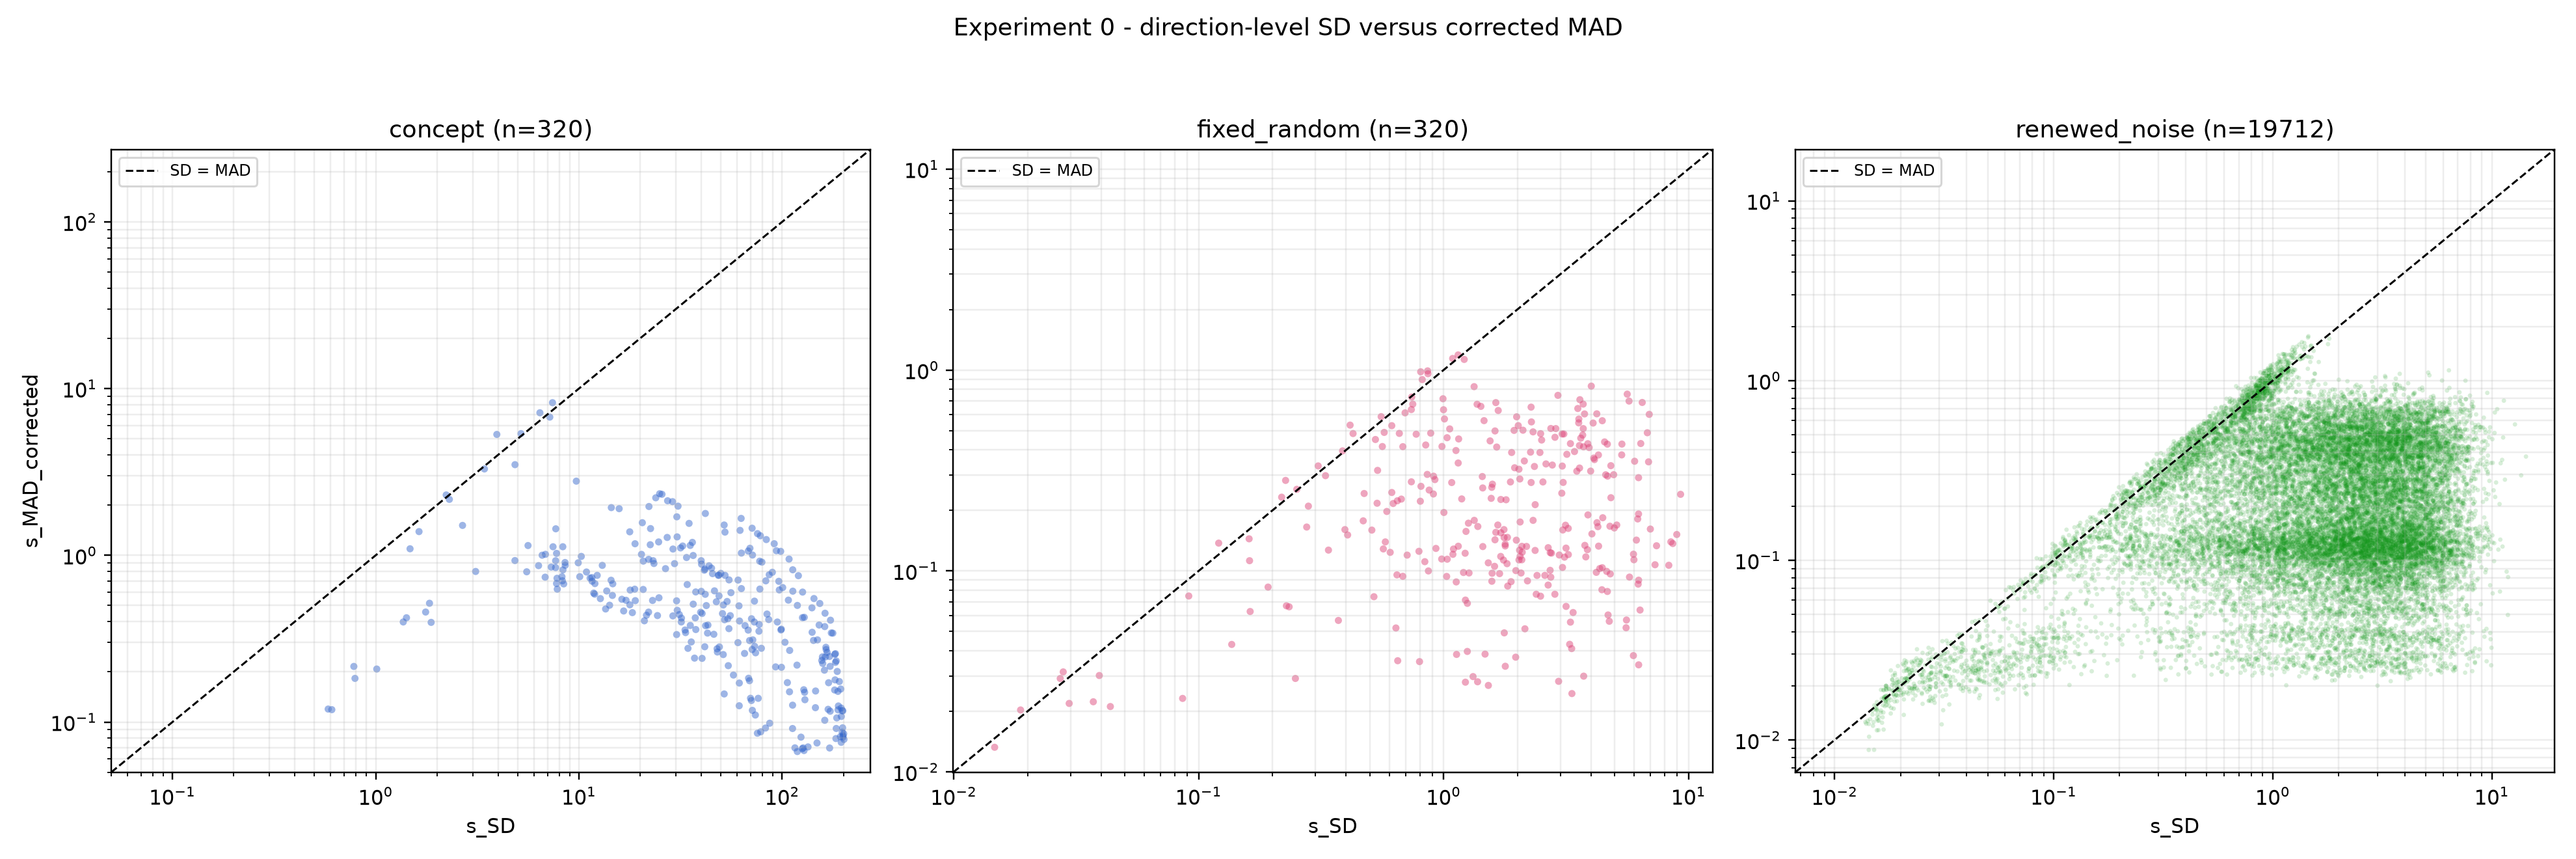
\includegraphics[width=0.68\textwidth]{experiment_0_sd_vs_mad.png}
  \par\vspace{0.3ex}
  {\footnotesize
  Comparaison de $s_{\mathrm{SD}}$ et de la MAD corrigée pour chaque couple
  $(\ell,v)$, séparément dans les trois familles. Les axes sont logarithmiques
  et la diagonale en pointillés représente $s_{\mathrm{SD}}=s_{\mathrm{MAD}}$.
  Un point sous la diagonale correspond à
  $s_{\mathrm{SD}}>s_{\mathrm{MAD}}$.\par}
\end{center}

La SD et la MAD corrigée ne fournissent pas des estimations équivalentes dans
les couches internes. Le rapport médian
\[
R(\ell)
=
\operatorname{médiane}_{v}
\frac{s_{\mathrm{SD}}(\ell,v)}
     {s_{\mathrm{MAD}}(\ell,v)}
\]
vaut, au bloc~1, environ $2\,355$ pour les concepts, $51$ pour les directions
aléatoires fixes et $76$ pour le bruit renouvelé. Au bloc~16, ces rapports
restent respectivement proches de $92$, $8{,}6$ et $12{,}4$. Ils diminuent
ensuite et deviennent proches de $1$ pour les trois familles au bloc~31.

Cette différence précise ce que mesurent les deux estimateurs. La SD dépend du
second moment de toute la distribution :
\[
s_{\mathrm{SD}}^2
=
\frac{1}{N-1}\sum_i(p_i-\overline p)^2.
\]
Elle augmente fortement lorsque certains groupes de projections sont éloignés
du centre. La MAD mesure au contraire la largeur de la moitié centrale de la
distribution :
\[
s_{\mathrm{MAD}}
=
1{,}4826\,\operatorname{médiane}_i
\left|p_i-\operatorname{médiane}(p)\right|.
\]
Une SD très élevée accompagnée d'une MAD faible signifie donc que la dispersion
globale est bien plus grande que la dispersion centrale.

Les résultats sont compatibles avec des distributions étroites dans leur région
centrale, mais comportant des groupes de projections plus éloignés. Plusieurs
mécanismes peuvent produire cette structure : mélange entre positions de tokens,
hétérogénéité entre phrases, multimodalité ou observations extrêmes. Le rapport
SD/MAD ne permet pas de choisir entre ces explications. Il montre en revanche
que l'hypothèse d'une distribution approximativement gaussienne n'est pas
valable dans une grande partie du réseau.

La divergence est particulièrement forte pour les directions conceptuelles.
Cela suggère que leur grande SD n'est pas due à un élargissement uniforme de
toutes les projections : une partie substantielle de la distribution reste
concentrée, tandis que d'autres observations portent une variance beaucoup plus
importante. Cette structure peut expliquer simultanément la forte échelle SD
des concepts et leur différence avec les directions isotropes.

Ces résultats ne démontrent pas que la MAD est meilleure que la SD, ni
l'inverse. Les deux estimateurs correspondent à deux définitions distinctes de
l'intensité naturelle :

\begin{itemize}
  \item la SD mesure la variabilité globale effectivement observée, y compris
        celle des groupes éloignés ;
  \item la MAD mesure une variabilité centrale typique, robuste à ces groupes.
\end{itemize}

La MAD ne peut dès
lors être traitée comme un contrôle secondaire susceptible de produire
nécessairement les mêmes résultats : elle constitue une véritable
paramétrisation alternative.

\subsection{Stabilité par bootstrap}

\begin{center}
  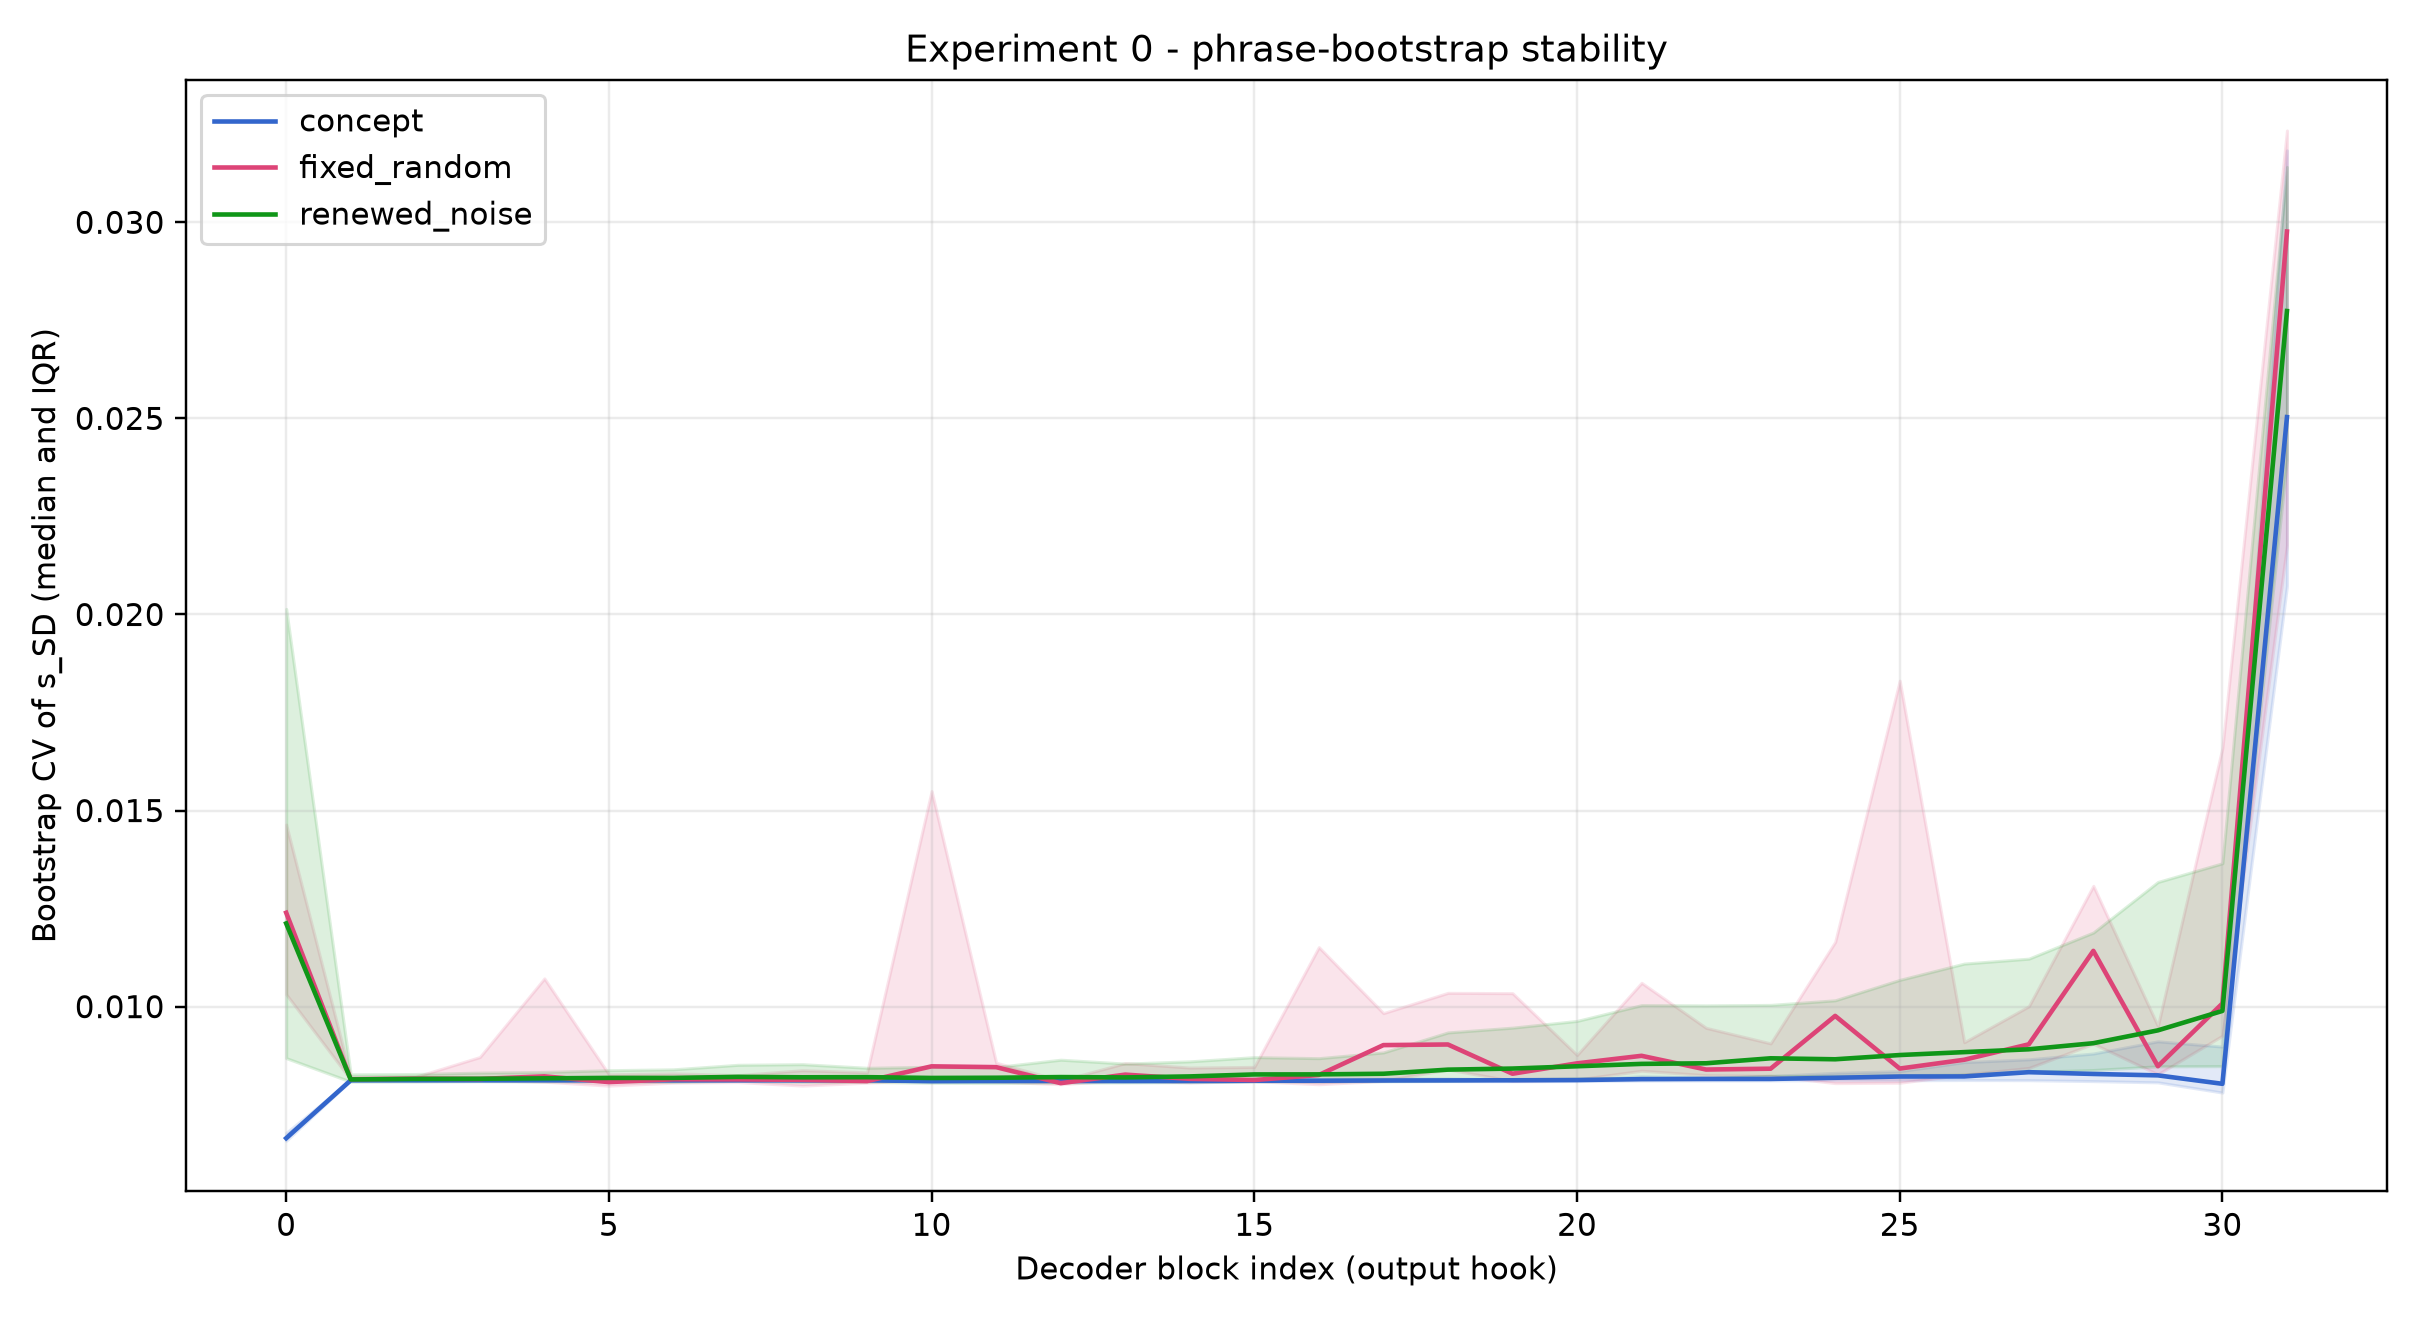
\includegraphics[width=0.48\textwidth]{experiment_0_bootstrap_stability.png}
  \par\vspace{0.3ex}
  {\footnotesize
  Coefficient de variation bootstrap de $s_{\mathrm{SD}}$. La ligne représente
  la médiane et la bande l'IQR entre les directions de chaque famille. Le
  bootstrap rééchantillonne les 100 phrases avec remise et conserve tous les
  tokens admissibles de chaque phrase sélectionnée.\par}
\end{center}

La divergence entre SD et MAD n'est pas accompagnée d'une forte instabilité de
la SD vis-à-vis du choix des phrases. Sur 1\,000 réplications bootstrap par
phrase, le coefficient de variation médian de $s_{\mathrm{SD}}$ est proche de
\pc{0,8} dans les trois familles. Le quantile à \pc{95} reste inférieur à
environ \pc{2,7}, et le maximum observé est inférieur à \pc{6,5}. La hausse
visible au dernier bloc demeure donc limitée en valeur absolue.

La forte SD des couches internes est ainsi reproductible lorsque l'on
rééchantillonne les phrases de ce corpus. Cela rend peu probable une explication
reposant uniquement sur une ou deux phrases accidentelles. Cette stabilité ne
valide cependant pas automatiquement la SD comme meilleure définition de
l'intensité : le bootstrap évalue l'incertitude de l'estimateur sous le même
protocole, mais ne teste ni une autre pondération des tokens, ni un autre
contexte de présentation, ni la pertinence scientifique de la quantité
estimée.

Le contraste entre une SD stable et une forte divergence SD/MAD suggère plutôt
une structure systématique des distributions, répétée à travers le corpus. Une
décomposition future de la variance entre phrases, entre positions et à
l'intérieur des phrases permettra de déterminer quelle composante produit les
grandes échelles conceptuelles.

\subsection{Conséquences pour les expériences comportementales}

Les résultats confirment qu'un appariement à amplitude brute ne suffit pas.
À $\alpha$ égal,
\[
z(\ell,v)=\frac{\alpha}{s(\ell,v)}
\]
est beaucoup plus faible dans une direction conceptuelle de forte variance que
dans une direction isotrope typique. Les expériences comparant concept,
direction aléatoire et bruit à $\alpha$ égal opposeraient donc des perturbations
très différentes relativement à la géométrie naturelle du modèle.

Réciproquement, un appariement à $z$ égal implique des amplitudes absolues
différentes :
\[
\alpha(\ell,v,z)=z\,s(\ell,v).
\]
Il neutralise la différence d'échelle directionnelle, mais peut conduire à des
coefficients très élevés pour certaines directions conceptuelles, surtout avec
la SD dans les couches précoces. Les futures grilles devront donc vérifier que
ces doses restent dans un régime comportemental exploitable et ne provoquent
pas simplement une saturation ou une dégradation générale du modèle.

L'analyse principale restera fondée sur $s_{\mathrm{SD}}$, conformément au
protocole annoncé, mais les conclusions devront être recalculées avec
$s_{\mathrm{MAD}}$. Trois situations seront distinguées :

\begin{itemize}
  \item si les conclusions sont similaires avec SD et MAD, elles seront robustes
        au choix de l'estimateur d'échelle ;
  \item si seule l'amplitude brute $\alpha$ produit une différence entre
        familles, celle-ci pourra être attribuée à leur géométrie naturelle ;
  \item si SD et MAD conduisent à des conclusions comportementales différentes,
        la détectabilité dépendra de la définition retenue pour l'intensité et
        aucune interprétation unique ne devra être privilégiée.
\end{itemize}




\section{Partie 5 --- Expérience 1 : localisation 2AFC sur Llama-3.1-8B}

Balayage \texttt{full32\_all} : 306\,280 essais, 32 blocs, 4 familles, 2 appariements.
Calibration en statut \texttt{development} --- ces chiffres ne sont pas sous protocole figé.

\subsection{L'indicateur à rapporter n'est pas l'\emph{accuracy}}

Le modèle répond \og A\fg{} dans \pc{98} des essais. L'\emph{accuracy} brute vaut 0,509 à toutes les
couches et à toutes les doses : \textbf{rien ici ne montre le modèle \emph{rapportant} où il a été
perturbé}. L'\emph{accuracy} ajustée (0,551) reste biaisée : sur les blocs vifs elle vaut 0,481
quand la cible est étiquetée A et 0,753 quand elle est étiquetée B, alors que les deux \emph{positions
physiques} sont indiscernables (0,6178 / 0,6164). L'écart tient à la lettre. Cause : perturber
n'importe quoi éloigne les logits de la réponse par défaut A (contraste ajusté moyen $-0{,}310$),
ce qui compte comme succès sur tout essai ciblant B.

Le bon estimateur est le contraste apparié de la section 5.8, déjà calculé sous le nom
\texttt{mean\_localization\_contrast} :
\[ S = \tfrac12\left[L(\text{A ciblée}) - L(\text{B ciblée})\right], \]
qui annule tout déplacement ne dépendant pas de \emph{quelle} phrase a été touchée.

\subsection{Résultat principal}

\begin{center}\small
\begin{tabular}{llrrrr}
\toprule
Appariement & Famille & $S$ moyen & IC \pc{95} hiér. & part $S>0$ & \emph{acc.} ajustée \\
\midrule
$\alpha$ & concept        & 0,301 & [0,225 ; 0,381] & 0,670 & 0,654 \\
$\alpha$ & bruit          & 0,294 & [0,240 ; 0,348] & 0,658 & 0,616 \\
$\alpha$ & \emph{dropout} & 0,287 & [0,240 ; 0,342] & 0,652 & 0,606 \\
$\alpha$ & aléatoire fixe & 0,230 & [0,167 ; 0,297] & 0,612 & 0,579 \\
\bottomrule
\end{tabular}
\end{center}

Blocs 0--13, bootstrap hiérarchique (directions puis paires de phrases). Tous les intervalles
excluent zéro, mais les quatre familles se chevauchent largement à $\alpha$ apparié.

\textbf{Coupure nette au bloc 14.} Les blocs 0--13 localisent ; les blocs 14--30 sont exactement au
hasard (0,4993 sur 164\,560 essais, égalités exclues) ; le bloc 31 est identiquement nul.
Ce n'est pas la perturbation qui s'estompe : sa magnitude décroît continûment avec la profondeur
(1,60 au bloc 0 ; 0,86 au bloc 13 ; 0,52 au bloc 14 ; 0,06 au bloc 30) alors que l'\emph{accuracy}
chute de 0,77 à 0,50 en un seul bloc. Ce qui disparaît est l'information sur \emph{quelle} phrase.
Le bloc 31 est structurellement mort : le \emph{hook} est sur la sortie du bloc, qui n'est plus
suivie que d'opérations positionnelles et ne peut atteindre le token de réponse.

\begin{center}
  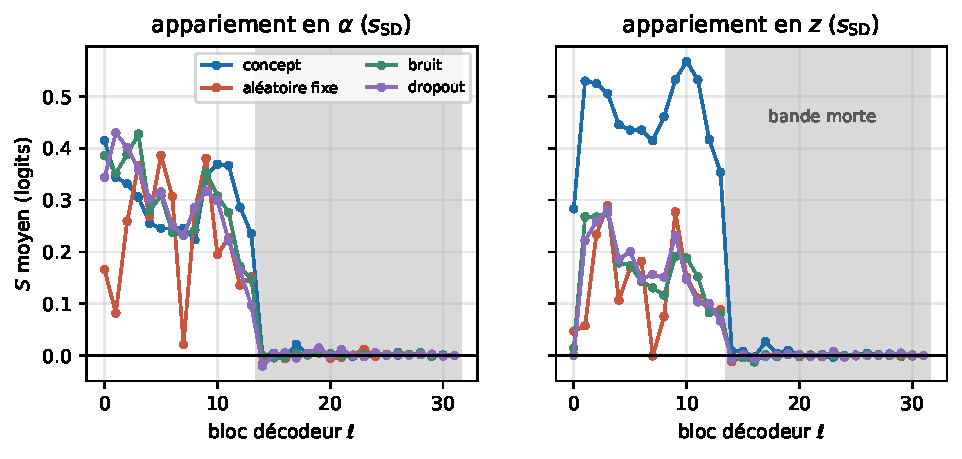
\includegraphics[width=0.86\textwidth]{experiment1-llama/depth_profile.pdf}
\end{center}

\begin{center}
  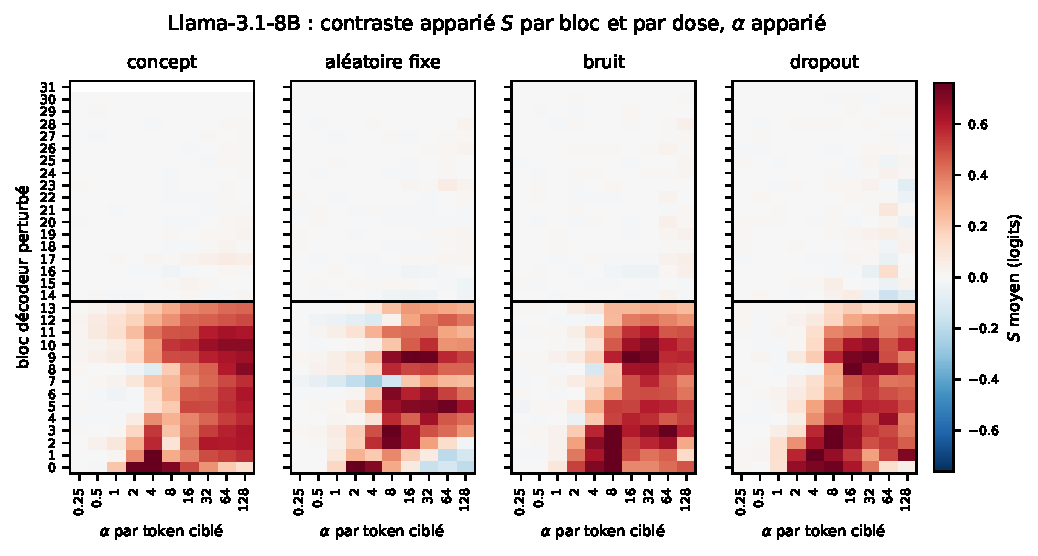
\includegraphics[width=0.97\textwidth]{experiment1-llama/heatmap_alpha.pdf}
\end{center}

La carte bloc\,$\times$\,dose rend la coupure visible d'un coup d'{\oe}il : au-dessus du trait,
tout est blanc à toutes les doses. Elle montre aussi que la famille conceptuelle atteint le régime
détectable à une dose plus faible (le front rouge y est décalé vers la gauche), et fait apparaître
les cellules \emph{bleues} de la famille aléatoire à doses faibles et moyennes. Ce sont les seules
cellules significativement \emph{sous} le hasard de tout le balayage : 13 sur 2\,794, toutes de
cette famille, toutes aux blocs 7 et 12, et aux deux appariements. La plus extrême,
\texttt{fixed\_random\_\_block\_07\_\_0000}, tombe à une \emph{accuracy} ajustée de 0,050 à
$\alpha = 1$ et à $\alpha = 2$. Une poussée cohérente à ces profondeurs déplace la réponse
vers la \emph{mauvaise} phrase ; le phénomène reste inexpliqué.

Cette carte n'est pas concernée par le défaut d'échelle de la section suivante : $\alpha$ est
l'amplitude physique par token, demandée puis réalisée, et aucune valeur calibrée n'entre dans son
calcul. Deux réserves de plan subsistent néanmoins, toutes deux dans les colonnes de droite.
Au-delà de $\alpha = 32$, le taux de \emph{dropout} vaut déjà 0,80 puis 0,92 et 0,976 : ces doses
ne sont plus des augmentations de dose mais une phrase déjà oblitérée, et l'amplitude réalisée
décroche (99,4 pour 128 demandé). Et les familles témoins étant non monotones, \og plus rouge vers
la droite\fg{} cesse d'être vrai en haut de grille.

\subsection{Contrôles nuls}

\textbf{Permutation.} En permutant au hasard, dans chaque paire, lequel des deux essais compte comme
\og A ciblée\fg{}, à logits et biais inchangés : $S$ observé $+0{,}3877$ contre un nul de
$-0{,}0001 \pm 0{,}0042$ sur 200 tirages (24\,640 paires), soit $92\sigma$. Le signal est
dans l'appariement perturbation/cible, pas dans le biais.

\textbf{Bande morte.} Le même pipeline rend $S = 0{,}000$--$0{,}003$ aux blocs 14--30. Un indicateur
qui fabriquerait du signal à partir d'un modèle biaisé en montrerait partout.

\textbf{Ordre de grandeur.} La marge A/B des sham vaut 1,725 logit ; la perturbation conceptuelle
déplace l'écart de 0,40 à 0,53, soit un quart. Assez pour être mesuré, pas pour renverser une
décision --- d'où une \emph{accuracy} brute clouée à 0,5 avec un $S$ élevé.

\subsection{Mesures de la section 5.14}

\begin{center}\small
\begin{tabular}{lr@{\qquad}lr}
\toprule
\emph{accuracy} brute / ajustée & 0,509 / 0,551 & Biais sham (20 conditions) & $+1{,}725$ logit, \pc{100} préfèrent A \\
Taux d'invalides & 0,008 & Taux d'égalités & 0,414 \\
Amplitude réalisée (additives) & exacte à $5\cdot10^{-5}$ & \emph{dropout} : $p$ à $\alpha=128$ & 0,976 (max 0,99994) \\
Seuils rapportables & \textbf{17 / 508} & $d'$, critère, AUROC & sans objet (expérience 2) \\
\bottomrule
\end{tabular}
\end{center}

Deux défauts de plan en découlent. \textbf{L'axe de dose du \emph{dropout} est dégénéré} au-dessus de
$\alpha = 32$ : $p$ ne peut dépasser 1, donc les doses supérieures ne sont plus des augmentations de
dose. \textbf{La forme psychométrique est fausse} : à $\alpha$ apparié, les 14 couches vives des
familles témoins culminent \emph{avant} la dose maximale puis redescendent (perte de 0,16 à 0,21),
alors que l'ajustement est une logistique monotone --- d'où seulement 17 seuils rapportables sur 508.
Le concept est nettement plus monotone (chute 0,049) : il sature, les témoins s'inversent.
\textbf{Aucun seuil à \pc{75} de ce balayage ne doit être cité.}

\textbf{Instabilité de l'ordre des étiquettes.} Un ré-étiquetage cosmétique --- mêmes phrases, même
ordre physique, même perturbation --- change $S$ d'un facteur 2,4 (AB : 0,379 ; BA : 0,160), alors
que l'ordre physique est parfaitement équilibré (0,271 / 0,268). Aucun chiffre unique n'est donc une
propriété stable du modèle.

\textbf{Contamination.} Le diagnostic $P_{1\rightarrow2}$ sature à 0,65--1,47 en deux blocs et ne
décroît jamais ; plusieurs cellules dépassent 1,0. Aux doses hautes la phrase non ciblée n'est plus
un témoin, et la question 2AFC est mal posée.

\subsection{L'appariement en $z$ est invalide : l'échelle est mesurée dans le mauvais contexte}

C'est le résultat méthodologique de cette partie.

L'expérience 0 calibre $s(\ell,v)$ sur des phrases rendues \textbf{isolément}
(\texttt{template: "\{sentence\}"}). Chaque phrase est alors sa propre séquence, et son premier token
occupe la \textbf{position 0} --- le puits d'attention, où Llama loge une activation massive. La
politique \texttt{all\_sentence\_tokens} l'inclut : il pèse \pc{16} de l'échantillon
($616/100 = 6{,}16$ tokens par phrase, soit exactement un par phrase). L'expérience 1 enchâsse les
mêmes phrases dans le prompt 2AFC, où les tokens perturbés sont aux positions ${\sim}40$--$80$ et
\textbf{aucun n'est jamais en position 0}.

Mesure directe des deux contextes, mêmes phrases et mêmes directions :

\begin{center}\small
\begin{tabular}{rlrrrr}
\toprule
& & \multicolumn{2}{c}{phrase isolée (calibrée)} & \multicolumn{2}{c}{prompt 2AFC (perturbé)} \\
\cmidrule(lr){3-4}\cmidrule(lr){5-6}
Bloc & Famille & $s_{\mathrm{SD}}$ & $s_{\mathrm{SD}}/s_{\mathrm{MAD}}$ & $s_{\mathrm{SD}}$ & $s_{\mathrm{SD}}/s_{\mathrm{MAD}}$ \\
\midrule
1  & concept   & 198,67 & 2451 & 0,0248 & \textbf{0,93} \\
1  & aléatoire & 3,55   & 141  & 0,0203 & \textbf{1,00} \\
13 & concept   & 146,98 & 429  & 0,2511 & \textbf{0,91} \\
13 & aléatoire & 1,62   & 12,6 & 0,1069 & \textbf{0,97} \\
\bottomrule
\end{tabular}
\end{center}

Pour \texttt{recursion} au bloc 1, en contexte isolé, la projection maximale vaut \textbf{582,3 en
position 0} et \textbf{0,399 partout ailleurs}. Dans le contexte comportemental la queue lourde
disparaît ($s_{\mathrm{SD}}/s_{\mathrm{MAD}} = 0{,}91$--$1{,}11$) et le rapport d'échelle
concept/aléatoire --- la quantité que la division par $s$ élimine --- tombe de \textbf{56--95} à
\textbf{1,2--2,4}.

\textbf{Ce n'est ni un défaut d'implémentation ni un problème de données.} SD est calculé
correctement, aucun BOS n'est ajouté, la bonne échelle va à la bonne famille. C'est le contexte de
présentation, que la configuration signale elle-même comme provisoire et que
\texttt{protocol\_config.py} refuse déjà au moment du gel.

\textbf{Piège à éviter.} \og Mettre les familles à la même amplitude physique\fg{} n'est pas le but
de l'appariement en $z$ --- c'est celui de l'appariement en $\alpha$. H1c énonce que $z$
\emph{modifie} les écarts vus à $\alpha$. Le défaut n'est pas l'inégalité des amplitudes, c'est que
$s$ a été estimée sur une distribution absente de l'expérience.

\textbf{Conséquence.} Les résultats en $z$ de ce balayage ne sont pas interprétables, ni pour
confirmer ni pour infirmer H1c. Les résultats en $\alpha$, qui n'appellent aucune échelle calibrée,
sont intacts.

\textbf{Correctif.} Recalibrer en contexte comportemental, via le mode \texttt{external\_manifest}
qui existe déjà. MAD n'est pas le correctif : dans le bon contexte $s_{\mathrm{SD}} \approx
s_{\mathrm{MAD}}$, et MAD redevient le simple contrôle de robustesse prévu. Défaut indépendant qui
survit à la recalibration : la grille $z$ plafonne encore à $\alpha \approx 5$ et doit être étendue.

\subsection{Les vecteurs conceptuels sont la direction de puits}

En cherchant la cause du rapport 56--95, une anomalie plus lourde apparaît. Le token de position 0
porte une norme d'activation de ${\sim}547$ contre 1,7--9,7 ailleurs. Cosinus absolu entre chaque
direction et cette direction de puits (attendu isotrope en dimension 4096 : $1/\sqrt{4096}=0{,}0156$) :

\begin{center}\small
\begin{tabular}{rrrrrr}
\toprule
Bloc & Dust & Satellites & recursion & shutdown & les 3 aléatoires \\
\midrule
1  & 0,982 & 0,632 & \textbf{0,994} & 0,983 & 0,011--0,027 \\
13 & 0,744 & 0,205 & 0,856 & 0,699 & 0,007--0,011 \\
\bottomrule
\end{tabular}
\end{center}

Les directions aléatoires tombent exactement sur l'attendu isotrope ; les conceptuelles en sont
\textbf{quasi colinéaires}. Les vecteurs sont des \emph{moyennes} d'états cachés
(\texttt{vec\_type: avg}), donc ils héritent de la composante d'activation massive, qui domine toute
moyenne par sa norme. Un vecteur à $|\cos| = 0{,}99$ ne garde que \pc{14} de sa norme dans un
sous-espace propre au concept.

Trois observations s'unifient : PC1 capte \pc{61}--\pc{83} de la variance entre les quatre vecteurs
conceptuels parce que \textbf{PC1 est la direction de puits, non un axe sémantique} ; Dust, seul
concept inerte ($S = 0{,}111$ contre 0,33--0,39), en est le pôle négatif ; Satellites est le moins
aligné et le seul dont le chargement PC1 soit nul. Le rapport d'échelle s'en déduit :
$0{,}86/0{,}0156 \approx 55$.

\textbf{Chantier distinct de la recalibration}, qui corrige $s(\ell,v)$ mais pas ce que \emph{sont}
les directions. Tant qu'il n'est pas traité, l'écart concept/témoins ne peut pas être attribué au
contenu conceptuel.

\subsection{Bilan}

\begin{itemize}
  \item \textbf{Affirmation défendable :} la perturbation déplace systématiquement les logits vers la
        phrase ciblée, d'environ un quart du biais de réponse permanent, et \emph{uniquement} dans
        les blocs 0--13. Pas de rapport comportemental.
  \item \textbf{Ordonnancement} concept $>$ bruit $\approx$ \emph{dropout} $>$ aléatoire, stable sous
        les trois paramétrisations. Son \emph{amplitude} varie d'un facteur 2,2 et n'est pas établie.
  \item \textbf{Non exploitable :} tous les résultats en $z$, tous les seuils à \pc{75}, et tout
        chiffre unique agrégé sur les deux ordres d'étiquettes.
\end{itemize}

\section{Partie 5\emph{bis} --- Expérience 1 sur Qwen3.8-27B}

Même protocole, modèle secondaire de la section 3.1. Blocs 3, 6, 8, 10, 12, 16, 32, 56 sur 64.
Calibration lancée depuis une config versionnée, donc sans \texttt{-{}-allow\_calibration\_mismatch}.
Statut \texttt{development} également.

\subsection{Sur ce modèle, la tâche 2AFC est une vraie tâche}

C'est le résultat inter-modèles le plus important. Bloc 3, concept, $\alpha$ apparié :

\begin{center}\small
\begin{tabular}{lrrrr}
\toprule
$\alpha$ & 8 & \textbf{16} & 32 & 64 \\
\midrule
\emph{accuracy} brute & 0,884 & \textbf{1,000} & 0,981 & 0,934 \\
taux d'égalités & 0,087 & 0,013 & 0,019 & 0,069 \\
\bottomrule
\end{tabular}
\end{center}

L'\emph{accuracy} brute est la lettre réellement émise. À $\alpha = 16$ le modèle nomme la phrase
ciblée dans \textbf{les 160 essais} de la cellule, et le seuil à \pc{75} sur la métrique brute vaut
$\alpha = 6{,}26$, encadré dans la grille.

La raison est dans le sham : le biais de réponse de Qwen vaut $+0{,}256$ logit (préférant A dans
\pc{85} des conditions) contre $+1{,}725$ pour Llama (\pc{100}). Le biais de Llama valait quatre fois
l'effet mesuré, d'où un argmax qui ne bascule presque jamais ; celui de Qwen en vaut un cinquième,
donc la décision bouge. \textbf{L'instrument qui ne se lisait qu'indirectement sur Llama se lit
directement ici.}

Second avantage : \textbf{le contrôle d'ordre des étiquettes passe}. AB : $S = 0{,}0593$ ; BA :
$0{,}0515$ --- \pc{15} d'écart, contre \pc{140} sur Llama.

\subsection{H1a --- déplacer l'injection déplace la réponse}

Validé largement. $S$ moyen, $\alpha$ apparié :

\begin{center}\small
\begin{tabular}{lrrrrr}
\toprule
Bloc & concept & aléatoire & bruit & \emph{dropout} & concept $\div$ aléatoire \\
\midrule
3  & $+0{,}3531$ & $+0{,}1828$ & $+0{,}1278$ & $+0{,}1598$ & 1,9$\times$ \\
6  & $+0{,}2124$ & $+0{,}0822$ & $+0{,}0699$ & $+0{,}0582$ & 2,6$\times$ \\
8  & $+0{,}1615$ & $+0{,}0693$ & $+0{,}0447$ & $+0{,}0236$ & 2,3$\times$ \\
10 & $+0{,}1313$ & $+0{,}0432$ & $+0{,}0581$ & $+0{,}0240$ & 3,0$\times$ \\
12 & $+0{,}0555$ & $+0{,}0554$ & $+0{,}0443$ & $+0{,}0138$ & \textbf{1,0$\times$} \\
16 & $+0{,}0400$ & $+0{,}0360$ & $+0{,}0291$ & $+0{,}0071$ & 1,1$\times$ \\
32 & $+0{,}0161$ & $-0{,}0217$ & $-0{,}0131$ & $-0{,}0165$ & --- \\
56 & $+0{,}0003$ & $+0{,}0006$ & $-0{,}0001$ & $-0{,}0001$ & --- \\
\bottomrule
\end{tabular}
\end{center}

Nul de permutation : $S$ observé $+0{,}0554$ contre $+0{,}0002 \pm 0{,}0013$, soit $41{,}4\sigma$.

\textbf{La bande vive est bien plus superficielle en profondeur relative.} Llama : blocs 0--13 sur
32, soit les \pc{44} premiers. Qwen : éteint dès le bloc 16 sur 64, soit les \pc{25} premiers. La
profondeur relative n'est \emph{pas} l'invariant entre modèles --- transposer un choix de couches par
proportion échantillonne surtout de la pile morte. La décroissance est douce : le concept perd
environ la moitié de son effet tous les cinq blocs.

La dernière colonne est plus intéressante : \textbf{l'avantage du concept sur une direction aléatoire
disparaît dès le bloc 12}, où les deux sont égaux à trois décimales alors que tous deux restent
au-dessus de zéro. Ce qui distingue une direction conceptuelle est une propriété des couches
précoces, pas de la pile. Le bloc 56 est un nul intégré ($|S| \leq 0{,}0007$, 81--\pc{88} d'égalités).

\begin{center}
  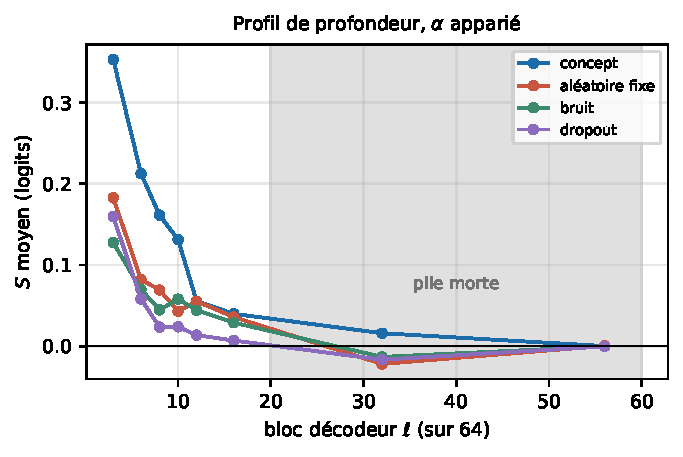
\includegraphics[width=0.62\textwidth]{experiment1-qwen/depth_profile.pdf}
\end{center}

\begin{center}
  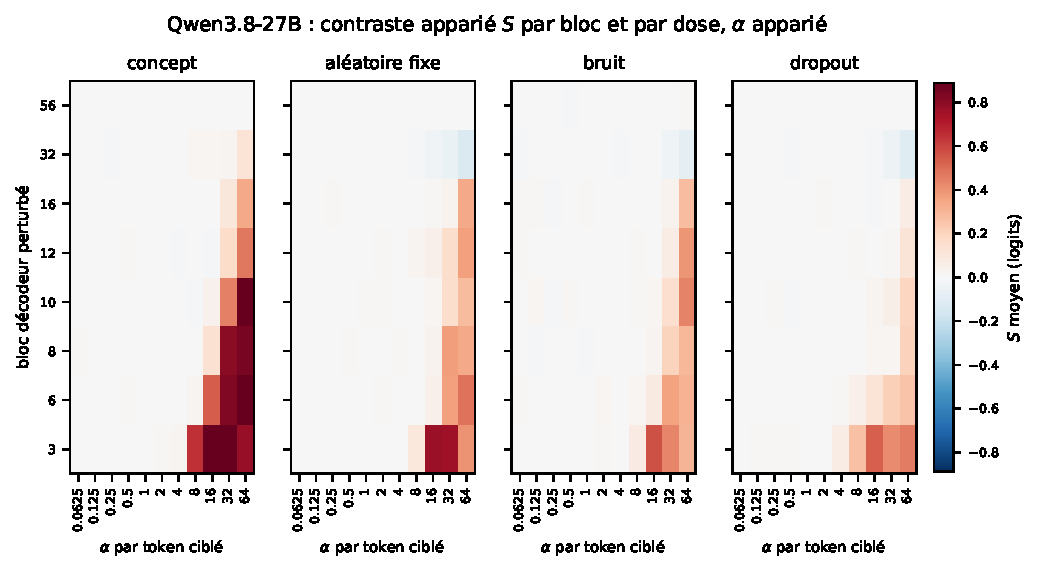
\includegraphics[width=0.97\textwidth]{experiment1-qwen/heatmap_alpha.pdf}
\end{center}

Mêmes conventions que pour Llama. Les blocs sondés n'étant pas équidistants (3, 6, 8, 10, 12, 16,
32, 56), les lignes sont à pas constant mais les profondeurs ne le sont pas. Le décalage du front
rouge vers la gauche pour le concept est la lecture visuelle de son avantage de seuil, et les
colonnes de gauche entièrement blanches montrent qu'aucune famille ne répond sous $\alpha \approx 8$.
Le liseré bleu au bloc 32 chez les trois témoins, absent chez le concept, est le renversement de
signe traité plus bas.

\subsection{H1b --- les familles diffèrent par le seuil, pas par la nature}

Au bloc 3, les \emph{accuracy} brutes maximales valent concept 1,000, aléatoire 0,996, bruit 0,925,
\emph{dropout} 0,925 : \textbf{toutes les familles atteignent le plafond} avec assez d'amplitude. Les
seuils à \pc{75} y valent concept \textbf{6,5}, \emph{dropout} 32,3, bruit 63,0, aléatoire encadré
dans [8 ; 16]. L'énoncé défendable est donc qu'une direction conceptuelle est détectée à un quart à un
dixième de l'amplitude requise par une direction générique --- pas que les directions génériques
soient indétectables.

\subsection{H1c --- confirmé comme énoncé, réfuté comme interprétation}

C'est la partie où la première version s'est trompée, et l'erreur était la version flatteuse.

Sur la grille $z$ publiée (plafond 20,48), pooling tous blocs : concept $+0{,}1016$
($t = 23{,}4$), \emph{dropout} $+0{,}0012$, bruit $+0{,}0005$, aléatoire $-0{,}0023$. Lu naïvement :
sous $z$ les témoins s'annulent tandis que le concept est intact --- la standardisation isolerait le
contenu conceptuel.

\textbf{C'était un artefact d'étendue de grille.} En comparant l'amplitude brute que la dose $z$
maximale délivre au seuil à \pc{75} de chaque famille mesuré sur la grille $\alpha$ :

\begin{center}\small
\begin{tabular}{rlrrr}
\toprule
Bloc & Famille & $\alpha$ délivré à $z = 20{,}48$ & seuil $\alpha$ (\pc{75}) & rapport \\
\midrule
3  & concept        & 87,6 & 6,3  & \textbf{14,0$\times$} \\
3  & aléatoire      & 3,7  & [8 ; 16] & \textbf{${\approx}0{,}3\times$} \\
6  & concept        & 74,5 & 11,6 & \textbf{6,4$\times$} \\
6  & \emph{dropout} & 2,1  & 40,5 & \textbf{0,05$\times$} \\
16 & aléatoire      & 10,3 & 54,5 & \textbf{0,19$\times$} \\
\bottomrule
\end{tabular}
\end{center}

La grille dépasse le seuil du concept de 6 à 14 fois et rate celui de chaque témoin de 5 à 20 fois.
\textbf{Aucun témoin n'a jamais été testé près de sa transition, à aucun bloc.}

Le balayage étendu ($z$ jusqu'à 655,36) tranche. Au bloc 3, aléatoire fixe : $S$ reste plat jusqu'à
$z = 20{,}48$ ($-0{,}005$, reproduisant exactement le résultat publié) puis transitionne juste
au-dessus : $+0{,}076$ à $z = 41$, $+0{,}515$ à 82, $+0{,}792$ à 164. \textbf{Toutes les familles
atteignent le plafond sous appariement en $z$} (\emph{accuracy} brute maximale 0,806--0,994 selon
famille et bloc).

\begin{center}
  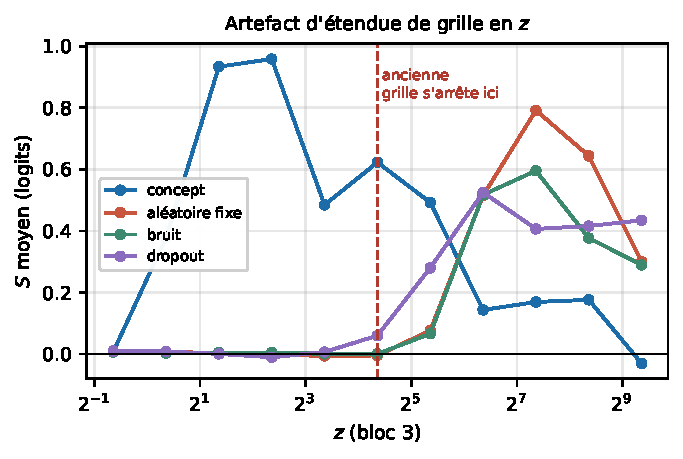
\includegraphics[width=0.62\textwidth]{experiment1-qwen/z_range_artefact.pdf}
\end{center}

Les témoins sont plats jusqu'à la limite de l'ancienne grille, puis transitionnent immédiatement
au-dessus. Les pics des familles sont distants d'un facteur ${\sim}30$ ($z \approx 5$ pour le
concept, $z \approx 164$ pour les témoins) : toute vue qui agrège une seule fenêtre de doses place
le concept dans sa décroissance à côté des témoins à leur pic, et affiche un écart
concept${-}$témoins \emph{négatif} qui est un artefact d'agrégation.

En clair, $z$ multiplie la séparation entre familles par le rapport de leurs échelles naturelles :
\[ \underbrace{40{,}1}_{\text{rapport des seuils en } z} = \underbrace{2{,}54}_{\text{rapport en }\alpha} \times \underbrace{15{,}8}_{\text{rapport des échelles}} \]
H1c est donc \textbf{confirmé comme énoncé} --- $z$ change bien les écarts, d'un facteur désormais
prédictible exactement --- et l'interprétation qu'il invite, un caractère catégoriel des directions
conceptuelles, est \textbf{réfutée}.

\subsection{Bloc 32 : les familles ont des signes opposés}

Pooling doses et appariements au bloc 32 : concept $+0{,}0213$ ($t = +8{,}2$), bruit $-0{,}0366$
($t = -12{,}1$), aléatoire $-0{,}0414$ ($t = -17{,}9$), \emph{dropout} $-0{,}0443$ ($t = -14{,}8$).
Le concept est significativement positif, les trois témoins significativement négatifs. Les deux
extrema sont à $\alpha = 64$, où une direction aléatoire éloigne la réponse de la phrase qu'elle
vise dans \pc{98,1} des paires qui bougent.

\textbf{Le contrôle \emph{scrambled} réfute la lecture par le contenu.} Une permutation des
coordonnées d'un vecteur conceptuel préserve exactement sa norme et le multiensemble de ses
coordonnées, mais détruit tout alignement avec une direction de \emph{feature}. C'est donc une
comparaison contenu contre magnitude, à magnitude tenue fixe par construction. Deux choses s'en
dégagent, et elles se séparent nettement :

\begin{center}\small
\begin{tabular}{rrrr@{\qquad}rrr}
\toprule
& \multicolumn{3}{c}{$S$ moyen, $\alpha$ apparié} & \multicolumn{3}{c}{échelle $s(\ell,v)$} \\
\cmidrule(lr){2-4}\cmidrule(lr){5-7}
Bloc & concept & \emph{scrambled} & aléatoire & concept & \emph{scrambled} & aléatoire \\
\midrule
3  & \textbf{$+0{,}4453$} & $+0{,}2545$ & $+0{,}2275$ & 2,779 & \textbf{0,172} & 0,176 \\
6  & \textbf{$+0{,}2999$} & $+0{,}0716$ & $+0{,}1281$ & 1,983 & \textbf{0,232} & 0,233 \\
12 & $+0{,}1122$ & $+0{,}0749$ & $+0{,}1115$ & 2,583 & \textbf{0,419} & 0,445 \\
32 & \textbf{$+0{,}0257$} & \textbf{$+0{,}0218$} & $-0{,}0270$ & 2,690 & \textbf{0,806} & 0,917 \\
\bottomrule
\end{tabular}
\end{center}

\textbf{Aux blocs superficiels, \emph{scrambled} retombe sur aléatoire} : le concept le devance de
1,75$\times$ au bloc 3 et 4,19$\times$ au bloc 6. L'avantage de seuil du concept porte donc sur
\emph{où pointe la direction}, et c'est du contenu au seul sens que ce plan peut tester. \textbf{Ce
résultat survit.} L'échelle le confirme avant tout essai : permuter effondre $s$ de ${\sim}2{,}7$ à
${\sim}0{,}17$, sur l'échelle aléatoire, à tous les blocs --- donc l'écart d'échelle de 16$\times$
qui pilote l'artefact en $z$ est un \emph{alignement réel} avec les directions de forte variance, pas
un artefact de construction.

\textbf{Au bloc 32, \emph{scrambled} se range du côté du concept} ($+0{,}0218$, $t = +7{,}5$), contre
aléatoire négatif ($t = -16{,}2$). Un vecteur conceptuel permuté ne porte aucun contenu et produit
pourtant le signe positif : \textbf{le signe ne suit pas le contenu}. La seule propriété que concept
et \emph{scrambled} partagent par construction, et qu'un tirage gaussien n'a pas, est la distribution
des coordonnées : kurtosis 8,3--8,5 contre 3,0, et dix coordonnées sur 5120 portant 7,7--\pc{8,0} de
l'énergie contre \pc{2,4}. Le signe au bloc 32 suit donc \textbf{le caractère à queue lourde de la
perturbation, pas sa signification}.

\begin{center}
  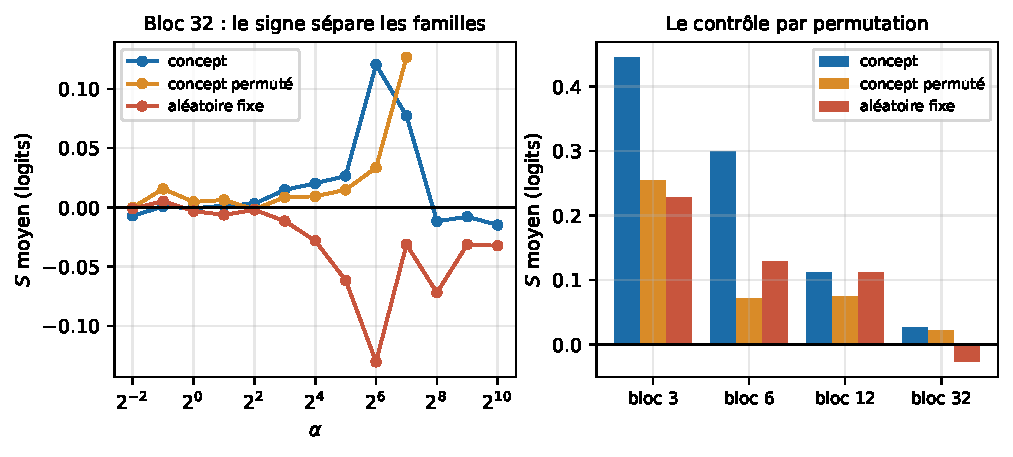
\includegraphics[width=0.92\textwidth]{experiment1-qwen/sign_split_scrambled.pdf}
\end{center}

À gauche, le bloc 32 : concept et concept permuté culminent tous deux positivement
($\alpha = 64$ et 128) tandis que l'aléatoire fixe plonge négativement au même endroit. À droite, la
permutation se comporte différemment selon la profondeur --- elle retombe au niveau de l'aléatoire
aux blocs 3 et 6, et se range du côté du concept au bloc 32.

\subsection{Autres mesures}

\textbf{Réponse non monotone.} Bloc 3, concept, $\alpha$ apparié : $S$ culmine à $\alpha = 16$
($+1{,}306$) puis redescend ($+1{,}111$ à 32 ; $+0{,}777$ à 64). Même forme pour aléatoire. Au-delà
de la saturation, la perturbation dégrade la représentation plus vite qu'elle ne localise. Les seuils
ci-dessus sont pris sur la branche montante et ne sont pas affectés, mais les deux doses hautes ne
doivent pas être données à un ajustement monotone.

\textbf{Contamination : un ordre de grandeur plus faible que sur Llama.} Médiane 0,067, maximum 0,229
sur les 32 relevés, contre 0,5--1,0 jusqu'au bloc 30 sur Llama (et $>1{,}0$ pour le \emph{dropout}).
Les deux phrases sont donc bien plus proches de deux observations indépendantes, même si 0,15 au bloc
16 n'est pas nul.

\subsection{Bilan et comparaison des deux modèles}

\begin{center}\small
\begin{tabular}{lll}
\toprule
& Llama-3.1-8B & Qwen3.8-27B \\
\midrule
Biais de réponse (sham) & $+1{,}725$ logit & $+0{,}256$ logit \\
\emph{Accuracy} brute maximale & 0,509 (plate partout) & \textbf{1,000} (bloc 3) \\
Lecture de l'instrument & indirecte (logits) & \textbf{directe (comportement)} \\
Bande vive & blocs 0--13 / 32 (\pc{44}) & blocs 3--12 / 64 (\pc{25}) \\
Contrôle ordre des étiquettes & \textbf{échoue} ($\times 2{,}4$) & passe ($\times 1{,}15$) \\
Contamination & 0,5--1,0, saturante & 0,067 médian \\
Queue lourde de $s$ ($s_{\mathrm{SD}}/s_{\mathrm{MAD}}$) & \textbf{506} (concept) & \textbf{1,2} (concept) \\
Appariement en $z$ & \textbf{invalide} (contexte de calibration) & exploitable, mais grille trop courte \\
\bottomrule
\end{tabular}
\end{center}

\textbf{Qwen est le meilleur instrument des deux}, sur les quatre critères qui comptent : le biais de
réponse, la lisibilité comportementale, la stabilité au ré-étiquetage et l'indépendance des deux
phrases. Les expériences 2 à 6 devraient être menées d'abord sur lui.

\textbf{Précision sur la dernière ligne du tableau.} Les deux modèles sont calibrés dans le
\emph{même} contexte de phrase isolée --- \texttt{qwen38\_27b\_full.yaml} porte le même
\texttt{context\_id: isolated\_sentence\_development} et le même avertissement que son homologue
Llama. Ce n'est donc pas la configuration qui les sépare, mais le modèle : le défaut décrit en
Partie~5 suppose que le modèle loge une activation massive en position~0, et \textbf{Qwen ne le fait
pas}. Le diagnostic, mesuré sur les deux calibrations :

\begin{center}\small
\begin{tabular}{lrrrr}
\toprule
& $s_{\mathrm{SD}}/s_{\mathrm{MAD}}$ concept & idem aléatoire & masse de queue $\times$ tokens/phrase & $s$ concept/aléatoire \\
\midrule
Llama-3.1-8B & \textbf{506} & 20,1 & \textbf{0,98} & 54,1 \\
Qwen3.8-27B  & \textbf{1,2} & 1,1  & \textbf{0,44} & 7,1 \\
\bottomrule
\end{tabular}
\end{center}

Une masse de queue de $0{,}98$ token par phrase signifie \emph{exactement un} token aberrant par
phrase --- le puits d'attention. À $0{,}44$, et avec $s_{\mathrm{SD}} \approx s_{\mathrm{MAD}}$
partout, les projections de Qwen sont proches d'une gaussienne et aucun token ne domine
l'échantillon. Son rapport d'échelle concept/aléatoire de $7$ à $16$ n'est donc pas un artefact de
puits, ce que le contrôle par permutation confirme indépendamment : permuter les coordonnées
effondre l'échelle sur celle de l'aléatoire.

\textbf{Réserve.} Ce diagnostic écarte l'artefact de puits sur Qwen ; il n'établit pas que l'échelle
en contexte isolé égale celle du prompt 2AFC. La sonde qui l'a vérifié sur Llama
(\texttt{code/analysis/probe\_calibration\_context.py}) n'a pas été rejouée sur le 27B. D'ici là,
\og exploitable\fg{} est le mot juste, pas \og valide\fg{}.

\textbf{Établi :} toutes les familles sont détectables sous les deux paramétrisations, avec assez
d'amplitude ; elles diffèrent par le seuil, pas par la nature. L'avantage du concept aux blocs
superficiels porte sur l'alignement et survit au contrôle par permutation.

\textbf{Non établi :} le compte par la queue lourde du signe au bloc 32 repose sur l'élimination.
Test direct, peu coûteux et non fait : une direction gaussienne remise à la distribution de
coordonnées des vecteurs conceptuels mais alignée sur rien.

\textbf{Deux erreurs corrigées en cours de route, enregistrées plutôt que corrigées en silence} : la
comparaison de familles en $z$, artefact d'étendue de grille, et l'interprétation du signe au bloc
32, réfutée par le contrôle \emph{scrambled}. Les deux pointaient dans la même direction --- celle
que ce projet aimerait trouver.


\end{document}
